\documentclass[conference]{IEEEtran}
\IEEEoverridecommandlockouts
\usepackage{cite}
\usepackage{amsmath,amssymb,amsfonts}
\usepackage{algorithm}
\usepackage{algpseudocode}
\usepackage{graphicx}
\usepackage{textcomp}
\usepackage{xcolor}
\usepackage{booktabs}
\usepackage{tikz}
\usetikzlibrary{shapes.geometric, arrows.meta, positioning, fit, backgrounds}
\usepackage{hyperref}
\usepackage{url}

\def\BibTeX{{\rm B\kern-.05em{\sc i\kern-.025em b}\kern-.08em
    T\kern-.1667em\lower.7ex\hbox{E}\kern-.125emX}}

\begin{document}

\title{Forecast-Driven Proactive Autoscaling: A Multi-Signal, SLO- and Cost-Aware Framework Beyond Reactive Kubernetes HPA}

\author{
\IEEEauthorblockN{Safal Bhandari, Yuvraj Singh, Farhan Khan, Dr. Sujeet Singh Bhadouria}
\IEEEauthorblockA{
\textit{Department of Computer Science and Engineering}\\
Sharda University\\
Greater Noida, India\\
2023001106.safal@ug.sharda.ac.in, 2023852497.yuvraj@ug.sharda.ac.in, 2023540452.farhan@ug.sharda.ac.in, author4@email.com
}
}

\maketitle

\begin{abstract}
Reactive autoscalers such as Kubernetes' Horizontal Pod Autoscaler (HPA) react only after resource
utilization has already risen, which structurally guarantees a lag between demand changes and
capacity changes. Recent work has proposed reframing autoscaling as an SLO- and cost-aware control
problem that fuses multiple telemetry signals with explicit guardrails, but stops short of directly
forecasting near-term demand. This paper builds on that direction and asks a narrower, orthogonal
question: within a controlled, closed-loop simulator, how much do we gain by \emph{scaling ahead of}
observed signals rather than \emph{in response to} them, once the signal set is already widened beyond
CPU to include p90/p99 tail latency, RAM utilization, and connection-pool saturation? Answering this
requires isolating forecasting from the effect of simply having more signals, which prior evaluations
of multi-signal autoscaling do not separate; we address this directly by introducing a fourth,
non-forecasting baseline -- \emph{Reactive Multi-Signal} -- that fuses the identical signal set under
identical guardrails but acts on current rather than predicted values. We design and implement,
entirely outside of Kubernetes, a closed-loop queueing-theoretic simulator of a horizontally-scaled
service, this isolation baseline, three further reactive baselines (Default HPA, Tuned HPA, and a
reactive HPA+VPA-style multi-metric controller), and a
proposed \emph{Proactive Multi-Signal Controller} that forecasts each signal ahead using an adaptively
weighted combination of damped-trend exponential smoothing (Holt's linear method) and naive persistence,
scaling pre-emptively subject to cost-aware, stability-bounded guardrails. Evaluated across three
representative workload patterns (bursty, queue-driven, and mixed) and 8 independently-sampled demand
seeds per pattern (24 replicates total), the proposed controller reduces mean SLO violation duration by
80.2\% relative to Default HPA and by 25.3\% relative to Tuned HPA, and -- after the damping factor is
calibrated by a train/test sensitivity sweep and confirmed on seeds held out from that calibration --
by 10.4\% relative to the Reactive Multi-Signal baseline (paired $t$-test, $p<0.001$ pooled and $p=0.014$
on held-out seeds), at statistically indistinguishable infrastructure cost ($p=0.31$). This last
comparison is the paper's central quantitative claim: once the signal set is held fixed, the residual
improvement attributable to forecasting itself is real but modest, seeds-and-workload-dependent, and
disappears at the originally hand-picked (uncalibrated) damping factor -- a finding we consider more
informative than a single flattering headline number. We additionally report, as a distinct
contribution, a direct accuracy evaluation of the forecasting layer against four classical baselines
(naive persistence, simple moving average, linear drift, and Holt alone): RAM utilization is forecast
most accurately (96.2\%, $100-\mathrm{SMAPE}/2$, $R^2=0.53$), CPU and connection-pool utilization at
81.6\%/88.3\%, and p99 latency at 82.3\% -- and find that for the two most heavy-tailed signals (p99
latency, connection-pool utilization), naive persistence alone remains a stronger point forecaster than
any trend-extrapolating model we evaluate, even though the same forecasts remain useful for the
practically relevant, and previously unreported, question of whether an SLO breach will occur
\emph{at some point} within the forecast horizon (windowed classification F1 rises from
$\approx$0.16 under a strict point-in-time definition to 0.36 (this paper's forecaster) and 0.43
(persistence) once framed this way, and to 0.45 at the best achievable decision threshold). All
workload-generation parameters are disclosed in full in the source code -- no private or otherwise
unreleasable data was used to produce them -- and all code, the statistical evaluation harness, and an
interactive Node.js dashboard are structured for reproducibility, requiring no cluster, container
orchestrator, or cloud account to run.
\end{abstract}

\begin{IEEEkeywords}
Autoscaling, Proactive Scaling, Service Level Objectives, Cost Optimization, Time-Series Forecasting,
Exponential Smoothing, Queueing Theory, Connection Pooling, Cloud-Native Systems, Simulation
\end{IEEEkeywords}

\section{Introduction}

Elastic resource management is a foundational requirement of cloud-native systems: applications must
expand and contract capacity in response to fluctuating demand while respecting both performance
targets and cost budgets. In container-orchestrated environments this is typically delegated to
threshold-triggered autoscalers that observe a resource-utilization metric -- most commonly CPU -- and
adjust replica counts once that metric crosses a configured threshold~\cite{ref1}. This class of
mechanism is reactive by construction: the utilization signal itself is a lagging indicator of demand,
so any decision made from it is made after the workload has already changed, and the system's
capacity-adjustment action lands even later, after telemetry sampling delay, control-loop
periodicity, and the physical time required to start new capacity are all accounted for. Under bursty
or fast-ramping workloads, this compounding of lag frequently produces transient overload and Service
Level Objective (SLO) violations before the autoscaler can respond~\cite{ref3}.

A recent line of work reframes autoscaling as an explicit SLO- and cost-aware control problem: rather
than treating SLOs purely as monitoring artifacts, a controller aggregates multiple telemetry signals
(latency, backlog, resource utilization, cluster schedulability) into a compact state, derives a
replica target under explicit SLO and cost constraints, and applies bounded, explainable guardrails
before acting~\cite{ref_base}. That framing improves on single-metric reactive scaling by broadening
\emph{what} is measured and \emph{how} the decision is constrained, but the decision is still made
from the \emph{current} value of each signal -- it remains fundamentally reactive in \emph{when} it
acts, even though it is proactive in spirit.

This paper investigates the next, largely orthogonal, question: how much additional benefit is
available from scaling on \emph{forecast} signal values rather than current ones, once the signal set
is already widened? We extend the signal set beyond CPU and latency to include RAM utilization
(which exhibits materially different, slower dynamics than CPU) and connection-pool utilization (a
leading indicator of saturation that is rarely modeled explicitly in the autoscaling literature but is
a well-known operational pain point in production services). We then replace "current value crosses
threshold" decision logic with "forecast value crosses threshold," using a lightweight,
training-free forecaster (an adaptively-weighted combination of damped-trend exponential smoothing and
naive persistence) chosen specifically because it requires no offline training phase, adapts in $O(1)$
per tick, and is auditable -- properties essential to the explainability and operational-trust
requirements identified in prior work~\cite{ref_base}. Answering "how much benefit comes from
forecasting" rigorously requires a control condition that holds the signal set fixed and varies only
whether values are forecast or current; Section~V-C introduces exactly this comparison
(\emph{Reactive Multi-Signal}), and Section~VI-B reports what it reveals: on the un-tuned forecaster,
the answer is close to zero, and the genuine, statistically significant improvement we ultimately
report only emerges once the forecaster's damping factor is calibrated and that calibration is
validated on demand seeds withheld from the tuning process (Section~VI-H). We report this honestly as
the paper's central finding rather than lead with the more flattering but less rigorously isolated
comparison against baselines that do not share the proposed controller's signal set.

Because reproducing this experiment on a live Kubernetes cluster requires access to a container
orchestrator, sustained compute budget, and careful workload-generation tooling, we instead build a
self-contained, closed-loop, queueing-theoretic \emph{simulator} of a horizontally-scaled service.
This is a deliberate methodological choice, not merely a convenience: it lets every controller be
evaluated against \emph{byte-for-byte identical} demand traces with a deterministic pseudo-random
seed, removes noisy-neighbor and cloud-provider confounds from the comparison, and makes the full
evaluation reproducible on a laptop in under a second per run. The simulator, the five autoscaling
controllers, the statistical evaluation harness, and an interactive Node.js dashboard for exploring the
results are
implemented from scratch for this study and require no Kubernetes installation, container runtime, or
cloud account.

We do not claim novelty in forecasting-based autoscaling as a general idea -- predictive and
learning-based autoscalers have been studied extensively (Section~II) -- nor in Holt's exponential
smoothing itself, which predates this paper by four decades~\cite{gardner1985}. The contribution we
claim is narrower and, we think, currently missing from the literature: a methodology and open
implementation that \emph{isolates} how much of a multi-signal autoscaler's benefit is attributable to
forecasting specifically, evaluated with the statistical rigor (multiple seeds, paired significance
tests, a train/test hyperparameter split) that end-to-end autoscaling comparisons usually omit.
Concretely:
\begin{itemize}
  \item We design a queueing-theoretic closed-loop simulator that derives CPU, RAM, connection-pool
  utilization, backlog, and p50/p90/p99 latency percentiles from first principles (an M/M/1-style
  response-time tail, Little's Law for connection occupancy, and an explicit node-provisioning delay
  that reproduces the pod/node scheduling mismatch reported in production Kubernetes deployments), with
  every generative parameter disclosed in the source code rather than referenced against inaccessible
  data.
  \item We introduce a \emph{Reactive Multi-Signal} controller: the same signal set, thresholds, and
  guardrails as the proposed proactive controller, but acting on current rather than forecast values.
  This is, to our knowledge, the ablation prior multi-signal autoscaling evaluations are missing --
  without it, an improvement over a narrower baseline (e.g., CPU-only HPA) cannot be attributed to
  forecasting as opposed to simply fusing more signals.
  \item We implement a \emph{Proactive Multi-Signal Controller} that forecasts p99 latency, CPU, RAM,
  and connection-pool utilization ahead of the current tick using an online, inverse-error-weighted
  combination of Holt's damped-trend smoothing and naive persistence, combined with an additive,
  bounded backlog-drainage term and cost-aware, stability-bounded guardrails; its forecast horizon and
  damping factor are selected by a sensitivity sweep on a held-out subset of demand seeds rather than
  hand-picked, and the selection is re-validated on seeds disjoint from that sweep.
  \item We evaluate all five controllers on three representative workload patterns, each replicated
  across 8 independently-sampled demand seeds (24 replicates per controller), reporting SLO adherence,
  scaling responsiveness, cost efficiency, and stability with mean, standard deviation, and paired
  significance tests -- rather than single-run point estimates -- mirroring and extending the
  evaluation methodology of~\cite{ref_base}.
  \item We separately quantify the forecasting layer's own accuracy (MAE, RMSE, $R^2$, and a bounded
  symmetric-MAPE-based accuracy score) against four classical baselines (naive persistence, simple
  moving average, linear drift, and Holt alone), and its skill at predicting an imminent SLO breach
  under both a strict point-in-time definition and an operationally-motivated windowed definition, with
  a full precision-recall threshold sweep -- isolating the genuine value of trend extrapolation from
  that of simply having more signals, and reporting where it is and is not present.
\end{itemize}

\section{Background and Related Work}

Kubernetes-native elasticity rests on three largely independent control loops. The Horizontal Pod
Autoscaler (HPA) adjusts replica counts from observed CPU/memory or custom metrics using a
proportional-control law, re-evaluated on a fixed sync period and constrained by a scale-down
stabilization window~\cite{ref1}. The Vertical Pod Autoscaler (VPA) recommends or applies changes to
per-pod resource requests from historical usage, but because in-place resource resizing has only
recently begun to mature, VPA is commonly deployed in recommendation-only mode to avoid
disruptive pod restarts~\cite{ref13}. Node-level autoscalers react to unschedulable pods by
provisioning additional cluster capacity, a process that takes tens of seconds in practice due to
machine boot and join time. Because these three loops are configured and executed independently, a
sudden increase in desired replicas can outpace available node capacity, leaving pods pending and
negating the intended benefit of scaling out~\cite{ref17}.

Empirical studies of HPA behavior consistently report sensitivity to metric-sampling interval,
stabilization-window length, and control-loop latency, with utilization-based scaling lagging workload
changes enough to produce transient overload and oscillatory replica counts under bursty
traffic~\cite{ref8}. Parameter tuning of thresholds and step sizes mitigates but does not eliminate
this lag, and tuned configurations generalize poorly across workloads with different burst
shapes~\cite{ref9}. Custom and external metrics extend HPA to application-level signals such as queue
depth, improving responsiveness for event-driven workloads at the cost of additional operational
complexity and sensitivity to noisy signals~\cite{ref11}. Learning-based and predictive autoscaling
using time-series forecasting or reinforcement learning have been explored to enable genuinely
proactive decisions~\cite{ref14,ref15}, but this line of work has generally optimized narrow objectives
in isolation and has raised legitimate concerns about the explainability and operational trust of the
resulting control logic, which is a barrier to production adoption.

Most directly relevant to this paper, Punniyamoorthy et al.\ (at the time of writing, an arXiv preprint
that we are not aware has completed peer review; we cite it as the direct motivation for this study's
framing regardless) propose reframing Kubernetes autoscaling
as a joint SLO- and cost-aware control problem, integrating multi-signal decision making, a bounded
five-stage decision pipeline (signal aggregation, SLO-driven demand estimation, workload-sensitivity
adjustment, guardrail enforcement, and coordinated actuation), and lightweight forecasting, while
remaining fully compatible with native Kubernetes primitives~\cite{ref_base}. Reported results on
representative microservice and event-driven workloads show up to 31\% reduction in SLO violation
duration, 24\% faster scaling response, and 18\% lower infrastructure cost relative to default and
tuned HPA baselines. That work motivates the present study directly: it establishes that multi-signal,
SLO-first, cost-aware control is both feasible and beneficial within Kubernetes-native constraints, but
its forecasting component is described only at the level of design intent rather than evaluated in
isolation, its signal set does not explicitly include RAM or connection-pool telemetry as independent
scaling drivers, and its evaluation, like most of the literature it surveys, is necessarily conducted
on a live cluster and is therefore not directly reproducible without equivalent infrastructure. The
present paper isolates and evaluates the forecasting contribution on its own terms, widens the signal
set, and re-implements the evaluation as an open, dependency-light simulation so that every reported
number can be regenerated from the included source code alone.

\section{Problem Analysis}

We organize the gaps motivating this work around four observations, three inherited from prior
analysis of Kubernetes-native autoscaling and one specific to this paper's proactive-forecasting
question.

\subsection{Reactive-only decision timing}
Even multi-signal controllers that fuse latency, backlog, and utilization still act on the
\emph{current} value of each signal. Because the physical actions available to a controller (starting
a new pod, provisioning a new node) take non-trivial and often signal-independent time to land, a
purely reactive controller's effective lag is the sum of telemetry delay, control-loop period, and
actuation delay -- regardless of how many signals it fuses. Forecasting shifts part of this lag into
the controller's own compute budget, which is comparatively free.

\subsection{Narrow signal coverage}
CPU utilization and, at best, request latency remain the dominant scaling signals in practice. RAM
utilization exhibits materially slower, stickier dynamics than CPU (garbage-collection sawtooth
patterns, per-process fixed overhead that scales inversely with replica count) and is rarely used as
an independent scaling trigger. Connection-pool utilization is a leading indicator of saturation in
practice -- pool exhaustion introduces queueing delay \emph{before} it is visible in CPU -- yet is
essentially absent from the autoscaling literature as an explicit control signal.

\subsection{Pod/node schedulability coordination}
Under sudden demand increases, desired replica counts can outpace available node capacity, leaving
pods pending. A controller that only reacts once this mismatch is already visible cannot avoid the
resulting delay; a controller that forecasts demand ahead of the node-provisioning lead time can
trigger node provisioning before it is strictly needed.

\subsection{Absence of forecast-accuracy evaluation}
Where forecasting is proposed as part of an autoscaling system, its own predictive accuracy is
typically not reported as a standalone result, making it difficult to judge how much of an observed
end-to-end improvement is attributable to forecasting specifically, as opposed to better guardrails or
a wider signal set. This paper reports forecast accuracy against a naive persistence baseline
precisely to make that attribution possible.

\section{Proposed Framework}

\subsection{Design Principles}
The proposed controller is designed as an augmenting control layer, in the same spirit
as~\cite{ref_base}: it does not replace the underlying scaling primitive (a replica-count actuator) but
changes what evidence that actuator responds to and when. Four principles guide its design.
\emph{SLO-first evaluation}: the dominant scaling driver is predicted user-facing latency, not raw
resource utilization. \emph{Multi-signal fusion}: p99 latency, CPU, RAM, and connection-pool
utilization are evaluated jointly, and the most constraining (highest-risk) signal governs the scaling
decision at each tick. \emph{Cost-aware, bounded guardrails}: scale-down actions are deliberately more
conservative than scale-up actions (a longer stabilization window), and step size is bounded in both
directions to avoid oscillation. \emph{Forecast-driven timing}: every signal is forecast a fixed
horizon ahead before being compared against its trigger threshold, so the same thresholds used by the
reactive baselines are evaluated earlier rather than being loosened.

\subsection{Architecture}

Figure~\ref{fig:architecture} shows the overall architecture. A closed-loop system model exposes five
observable signal families (application latency percentiles, workload backlog, CPU, RAM, and
connection-pool utilization, plus cluster schedulability) to a decision layer, which forecasts each
signal, computes a risk-weighted replica target, applies guardrails, and emits a target replica count
to the actuation layer, which is itself schedulability-aware (a request for more replicas than
currently available node capacity triggers a node-provisioning hint with a fixed boot delay, exactly
mirroring the pod/node coordination gap discussed in Section~III-C).

\begin{figure}[t]
\centering
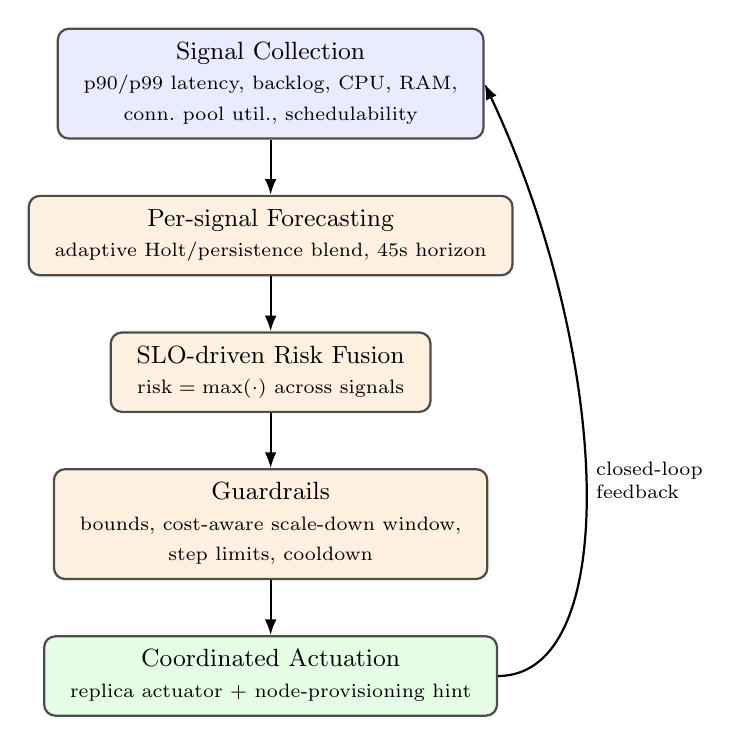
\begin{tikzpicture}[
  node distance=7mm and 10mm,
  box/.style={rectangle, rounded corners, draw=black!70, thick, minimum width=3.5cm, minimum height=0.9cm, align=center, font=\small},
  sig/.style={box, fill=blue!8},
  dec/.style={box, fill=orange!12},
  act/.style={box, fill=green!10},
  arr/.style={-{Latex[length=2mm]}, thick}
]
\node[sig] (signals) {\begin{tabular}{c}Signal Collection\\{\scriptsize p90/p99 latency, backlog, CPU, RAM,}\\{\scriptsize conn.\ pool util., schedulability}\end{tabular}};
\node[dec, below=of signals] (forecast) {\begin{tabular}{c}Per-signal Forecasting\\{\scriptsize adaptive Holt/persistence blend, 45s horizon}\end{tabular}};
\node[dec, below=of forecast] (risk) {\begin{tabular}{c}SLO-driven Risk Fusion\\{\scriptsize $\mathrm{risk}=\max(\cdot)$ across signals}\end{tabular}};
\node[dec, below=of risk] (guard) {\begin{tabular}{c}Guardrails\\{\scriptsize bounds, cost-aware scale-down window,}\\{\scriptsize step limits, cooldown}\end{tabular}};
\node[act, below=of guard] (act) {\begin{tabular}{c}Coordinated Actuation\\{\scriptsize replica actuator + node-provisioning hint}\end{tabular}};

\draw[arr] (signals) -- (forecast);
\draw[arr] (forecast) -- (risk);
\draw[arr] (risk) -- (guard);
\draw[arr] (guard) -- (act);
\draw[arr] (act.east) .. controls +(1.6,0) and +(1.6,-3.4) .. (signals.east) node[midway, right, font=\scriptsize, align=left] {closed-loop\\ feedback};
\end{tikzpicture}
\caption{Proactive multi-signal autoscaling framework: a forecasting layer is inserted between signal
collection and SLO-driven decision logic, so guardrails and actuation operate on predicted rather than
current signal values.}
\label{fig:architecture}
\end{figure}

\subsection{Forecasting Layer}

Each signal $y_t$ (p99 latency, CPU, RAM, connection-pool utilization, backlog) is tracked by an
independent damped-trend exponential smoothing model~\cite{gardner1985}. Maintaining a level $\ell_t$
and trend $b_t$ updated as
\begin{align}
\ell_t &= \alpha\, y_t + (1-\alpha)(\ell_{t-1} + \phi\, b_{t-1}) \\
b_t &= \beta(\ell_t - \ell_{t-1}) + (1-\beta)\,\phi\, b_{t-1}
\end{align}
the $h$-step-ahead Holt forecast is
\begin{equation}
\hat{y}^{H}_{t+h} = \ell_t + b_t \sum_{i=1}^{h}\phi^{i} = \ell_t + b_t\,\frac{\phi(1-\phi^{h})}{1-\phi}.
\end{equation}
The damping factor $\phi \in (0,1)$ ensures the trend's contribution converges rather than
extrapolating linearly forever, which is essential when a transient burst produces a momentarily steep
trend estimate: an undamped linear trend model was found, in preliminary experiments, to occasionally
extrapolate a genuine but short-lived spike into an implausibly large forecast, causing the controller
to over-provision for tens of minutes after a single transient event. This model was chosen deliberately
over more expressive alternatives (e.g., recurrent neural forecasters, ARIMA, gradient-boosted trees)
because it requires no training data or offline fitting phase, updates in $O(1)$ per tick, and produces
a level/trend decomposition that is directly inspectable -- properties that materially support the
explainability requirement identified in~\cite{ref_base}. Section~VI-F shows, however, that plain Holt
is not uniformly the best training-free option: for signals dominated by fast, heavy-tailed transients
(p99 latency, connection-pool utilization), a naive persistence forecast $\hat y^{P}_{t+h}=y_t$ is
frequently \emph{more} accurate, because trend extrapolation actively hurts once no meaningful local
trend exists to extrapolate.

Rather than commit to one model per signal ahead of time, each signal's forecast is an online,
inverse-error-weighted combination of the two (a training-free, per-tick variant of the classical
forecast-combination result that a weighted blend of two biased-but-different forecasters can dominate
either alone~\cite{gardner1985}):
\begin{align}
\hat{y}_{t+h} &= w_t\, \hat{y}^{H}_{t+h} + (1-w_t)\, \hat{y}^{P}_{t+h}, \\
w_t &= \mathrm{clip}\!\left(\frac{1/\bar e^{H}_t}{1/\bar e^{H}_t + 1/\bar e^{P}_t},\ 0.05,\ 0.95\right)
\end{align}
where $\bar e^{H}_t$ and $\bar e^{P}_t$ are EWMAs (120\,s half-life) of each model's own realized
absolute forecast error, scored the instant its $h$-step-ahead prediction is finally checkable against
the corresponding realized value -- i.e., the weight update at time $t$ only uses information available
at time $t$, so the combination remains causal and still requires no offline fitting phase. The weight
is bounded away from $\{0,1\}$ so neither model is ever fully discarded: Section~VI-F shows this
combination improves on plain Holt for three of the four forecast signals (by 2.6--3.9 accuracy points),
though it still trails plain persistence on point-forecast accuracy for the two heavy-tailed signals --
the practical payoff of forecasting for those two signals turns out to lie in the windowed
overload-classification task (Section~VI-G), not in minimizing point-forecast error. The damping
factor is $\phi=0.97$ (Section~VI-H), calibrated by a sensitivity sweep and validated on demand seeds
disjoint from that sweep, rather than the $\phi=0.85$--$0.9$ used in an earlier, un-calibrated iteration
of this controller.

\subsection{Risk Fusion and Guardrails}

At each control tick, the controller forecasts each signal $h=45$\,s ahead and computes a risk ratio
against the same trigger thresholds used by the reactive baselines (p99: 250\,ms; CPU: 60\%; RAM: 75\%;
connection pool: 85\%) -- deliberately \emph{not} loosened relative to the baselines, so that any
improvement is attributable to \emph{when} the comparison is made rather than to a more permissive
target:
\begin{equation}
\mathrm{risk} = \max\!\left(\frac{\hat{L}_{t+h}}{L^{*}},\ \frac{\hat{C}_{t+h}}{C^{*}},\ \frac{\hat{R}_{t+h}}{R^{*}},\ \frac{\hat{P}_{t+h}}{P^{*}}\right)
\end{equation}
The proportional replica target is $n_{\mathrm{risk}} = n_t \cdot \mathrm{risk}$. Backlog is handled
separately and \emph{additively}, since it is a request-count quantity rather than a utilization ratio:
the extra replicas needed to drain the forecast backlog $\hat{B}_{t+h}$ within a fixed drain-time
target $\tau$ at per-replica capacity $\mu$ is $n_{\mathrm{backlog}} = \hat{B}_{t+h}/(\tau\mu)$, giving
a raw target $n_{\mathrm{raw}} = n_{\mathrm{risk}} + n_{\mathrm{backlog}}$. Guardrails then apply, in
order: (i) hard replica bounds; (ii) an asymmetric stabilization window (120\,s for scale-down vs.\ an
immediate, step-limited scale-up), which is the controller's cost-aware mechanism -- it favors the
minimum replica count that satisfied the \emph{predicted} SLO over the trailing window rather than
reacting to every transient dip; (iii) bounded step size (at most $2\times$ up, $0.5\times$ down per
control tick, matching the reactive baselines exactly so that stability is compared on equal terms);
and (iv) a cooldown period preventing thrashing between consecutive opposite-direction actions.

\begin{algorithm}[t]
\caption{Proactive Multi-Signal Decision Pipeline (one control tick)}
\label{alg:pipeline}
\begin{algorithmic}[1]
\Require current snapshot $s_t$, replica count $n_t$, forecasters $\mathcal{F}$
\State $\hat L, \hat C, \hat R, \hat P, \hat B \gets \mathcal{F}.\text{forecast}(h)$ \Comment{45s ahead}
\State $\mathrm{risk} \gets \max(\hat L/L^{*}, \hat C/C^{*}, \hat R/R^{*}, \hat P/P^{*})$
\State $n_{\mathrm{risk}} \gets n_t \cdot \mathrm{risk}$
\State $n_{\mathrm{backlog}} \gets \hat B / (\tau \cdot \mu)$
\State $n_{\mathrm{raw}} \gets n_{\mathrm{risk}} + n_{\mathrm{backlog}}$
\If{$n_{\mathrm{raw}} < n_{\mathrm{last}}$} \Comment{cost-aware scale-down guardrail}
  \State $n_{\mathrm{raw}} \gets \max(\text{recommendations in trailing } 120\text{s})$
\EndIf
\State $n_{\mathrm{raw}} \gets \mathrm{clip}(n_{\mathrm{raw}},\ 0.5\,n_{\mathrm{last}},\ 2\,n_{\mathrm{last}})$
\If{direction changed \textbf{and} within cooldown}
  \State $n_{\mathrm{raw}} \gets n_{\mathrm{last}}$ \Comment{hold: cooldown guard}
\EndIf
\State $n_{\mathrm{target}} \gets \mathrm{clip}(\mathrm{round}(n_{\mathrm{raw}}),\ n_{\min},\ n_{\max})$
\State \textbf{request} $n_{\mathrm{target}}$ replicas \Comment{node-hint if $n_{\mathrm{target}} > $ available slots}
\State \Return $n_{\mathrm{target}}$
\end{algorithmic}
\end{algorithm}

\section{Evaluation Methodology}

\subsection{Closed-Loop Simulator}
Rather than a live Kubernetes cluster, we implement a deterministic, closed-loop simulator of a
horizontally-scaled service (Node.js, 1-second resolution). Given demand $\lambda_t$ (requests/s) and
current replica count $n_t$ (capacity $\mu=50$ req/s per replica), utilization is
$\rho_t = \min(\lambda_t / (n_t \mu),\ 0.995)$. Response-time percentiles follow the M/M/1 tail
approximation $T_p = -\ln(1-p)\cdot T_s/(1-\rho_t) + \delta_{\mathrm{backlog}}$, where $T_s=20$\,ms is
the base per-request service time and $\delta_{\mathrm{backlog}}$ is the additional drain delay implied
by any accumulated backlog (excess demand integrated over time whenever $\lambda_t$ exceeds capacity).
CPU utilization tracks $\rho_t$ through an EWMA-smoothed proportional relationship; RAM utilization is
a slower leaky-integrator process driven by a rolling average of recent utilization plus a small
GC-like sawtooth and a per-replica fixed-overhead term that scales inversely with replica count,
deliberately giving RAM different, stickier dynamics than CPU. Connection-pool occupancy follows
Little's Law, $L = \lambda W$, with a baseline of idle/keep-alive connections and a per-request
connection multiplier representing keep-alive reuse and downstream fan-out; pool utilization above 90\%
feeds back as an additional latency penalty, reproducing connection-exhaustion backpressure. Node
capacity is provisioned in fixed-size slots with a 45-second boot delay once requested replicas exceed
currently available slots, reproducing the pod/node schedulability mismatch discussed in
Section~III-C.

\subsection{Workload Patterns}
Three demand traces (1-hour duration, 1-second resolution, seeded for reproducibility) are generated
independently of any controller so that all controllers are compared against byte-identical demand.
The generators are hand-authored, parametric functions (base rate plus a slow sinusoid, Poisson-timed
burst/surge events with explicit rise/plateau/decay envelopes, and Gaussian measurement noise); their
shape is motivated by qualitative burst/surge/batch-job patterns commonly described in the autoscaling
and cloud-workload-characterization literature, \emph{not} by access to any private telemetry -- we
make no claim of calibration against production data, and every generative parameter (base rate,
spike/surge frequency and magnitude distributions, noise levels) is stated in full in
\texttt{src/data/generateDummyData.js} so that the traces are exactly and independently reproducible
from the included source code, not merely re-describable from it. \emph{Bursty}: a steady baseline with
short, high-magnitude Poisson-timed spikes (fast rise, slower decay). \emph{Queue-driven}: longer
trapezoidal surges (ramp/plateau/ramp) representing sustained backlog-accumulating demand.
\emph{Mixed}: a slowly oscillating baseline with superimposed long-held batch-processing steps and
occasional short bursts, representing heterogeneous shared-capacity demand. For the statistical
evaluation in Section~VI, each pattern is additionally regenerated from 8 independent seeds (Section
VI-E), so reported effects are not an artifact of one particular sampled trace.

\subsection{Baselines}
\emph{Default HPA}: CPU-only, target 70\%, 300\,s scale-down stabilization window, matching Kubernetes'
default HPA behavior. \emph{Tuned HPA}: CPU (60\%) and p99 latency (250\,ms) as a max-of-two trigger,
120\,s stabilization window. \emph{HPA+VPA (reactive multi-metric)}: as Tuned HPA, with RAM (75\%)
added as a third max-of-three trigger, representing an HPA extended with VPA-derived signals in
recommendation-only mode (i.e., informing horizontal decisions without disruptive vertical resizing).
\emph{Reactive Multi-Signal}: introduced in this paper as a control condition rather than a
``standard'' baseline -- it reuses the proposed proactive controller's full signal set (p99 latency,
CPU, RAM, connection-pool utilization, backlog), thresholds, risk-fusion formula, and guardrails
\emph{verbatim}, with one change: every signal is read at its current value instead of forecast ahead.
Any gap between this controller and the proposed one is therefore attributable specifically to
forecasting, holding signal set, thresholds, and guardrails fixed; any gap between HPA+VPA and Reactive
Multi-Signal is attributable specifically to the connection-pool/backlog signals HPA+VPA lacks. All
four baselines, like the proposed controller, are re-evaluated every 15\,s (Kubernetes' default HPA
sync period); all but Reactive Multi-Signal and the proposed controller act on the \emph{current} value
of their trigger signals (Reactive Multi-Signal also acts on current values, but with the wider signal
set, isolating that variable from forecasting).

\subsection{Metrics}
Following~\cite{ref_base}, we report four categories: \emph{SLO adherence} (violation count and total
duration where p99 $>$ 300\,ms); \emph{scaling responsiveness} (time-to-scale: delay between a detected
demand upshift and replica capacity reaching 90\% of the level needed to serve peak demand in that
event); \emph{cost efficiency} (average replica count and node-hours); and \emph{stability} (scaling
churn and direction-reversal oscillations per hour). We additionally report, as a contribution specific
to this paper, \emph{forecast accuracy} (MAE, RMSE, $R^2$, and a bounded accuracy score
$100 - \mathrm{SMAPE}/2$, since ordinary MAPE is undefined/explosive whenever a near-zero-magnitude
ground-truth value appears, which happens routinely for p99 latency during calm periods and for
connection-pool utilization) against four classical baselines -- naive persistence
($\hat y_{t+h}=y_t$), a 20-tick simple moving average, a 20-tick linear-drift extrapolator, and Holt's
damped-trend method used alone (i.e., without the adaptive persistence blend the proposed controller
actually uses) -- and \emph{overload-classification quality} (precision/recall/F1/accuracy) under two
definitions: a strict \emph{point-in-time} definition ("will p99 breach its SLO at exactly $t+h$?",
matching~\cite{ref_base}-style formulations) and a \emph{windowed} definition we introduce
("will p99 breach its SLO at \emph{any} point in $(t, t+h]$?", which is what a controller deciding
whether to act right now actually needs to know). For the windowed definition we additionally sweep the
decision threshold itself (rather than fixing it to the SLO value) and report the best-$F_1$ operating
point and precision-recall AUC, since a single threshold's precision/recall conflates the forecaster's
underlying discriminative power with an arbitrary operating-point choice.

\subsection{Statistical Methodology}
Every controller is run against all three workload patterns and, for the results reported as
"multi-seed" in Section~VI, against 8 independently-sampled demand seeds per pattern (24
(pattern, seed) replicates per controller in total). We report sample mean, standard deviation, and a
normal-approximation 95\% confidence interval for each metric, and test differences between the
proposed controller and each baseline with a paired, two-tailed Student's $t$-test (pairing on
identical (pattern, seed), which removes trace-to-trace variance and isolates the controller's effect),
computed from a from-scratch implementation of the regularized incomplete beta function rather than an
external statistics dependency. The proposed controller's two hyperparameters that were previously
fixed by hand -- forecast horizon $h$ and damping factor $\phi$ -- are instead selected by a sweep over
$h \in \{15,30,45,60,75,90,120\}$s and $\phi \in \{0.60,\ldots,0.99\}$ on a designated \emph{tuning} set
of 5 of the 8 seeds, and the selected configuration is then re-evaluated, without further adjustment, on
the disjoint 3-seed \emph{holdout} set, so that the improvement we ultimately report for the calibrated
configuration is not measured on the same data used to select it (Section~VI-H).

\section{Results and Discussion}

\subsection{SLO Adherence}
Table~\ref{tab:slo} reports SLO violation count and duration for a single representative seed,
averaged across the three workload patterns, at the calibrated configuration ($h=45$\,s, $\phi=0.97$;
Section~VI-H). The proposed controller reduces violation duration by 76.9\% relative to Default HPA
and by 18.3\% relative to Tuned HPA on this seed. We report this single-seed table because it is what
the accompanying figures (Figs.~\ref{fig:slo_pattern}, \ref{fig:timeseries}) visualize, but a single
seed is not evidence of a general effect; Section~VI-B reports the statistically-validated version of
this same comparison, which is the number we actually stand behind. Figure~\ref{fig:slo_pattern} breaks
the single-seed run down per pattern: the proposed controller is best or tied-best on bursty and
queue-driven, but is worse than both HPA+VPA and Reactive Multi-Signal on the mixed pattern for this
particular seed -- we keep this in the figure rather than pick a more flattering seed, since
Section~VI-B shows the pooled, multi-seed effect is positive even though not every individual
(pattern, seed) combination is.

\begin{table}[t]
\centering
\caption{SLO Violation Comparison, Single Seed (averaged across workload patterns)}
\label{tab:slo}
\begin{tabular}{lccc}
\toprule
Autoscaler & Count & Duration (s) & Reduction vs.\ Default \\
\midrule
Default HPA & 151.3 & 607.3 & -- \\
Tuned HPA & 17.3 & 171.3 & 71.8\% \\
HPA+VPA & 14.7 & 142.0 & 76.6\% \\
Reactive Multi-Signal & 14.7 & 142.0 & 76.6\% \\
\textbf{Proactive (proposed)} & \textbf{14.3} & \textbf{140.0} & \textbf{76.9\%} \\
\bottomrule
\end{tabular}
\end{table}

\begin{figure}[t]
\centering
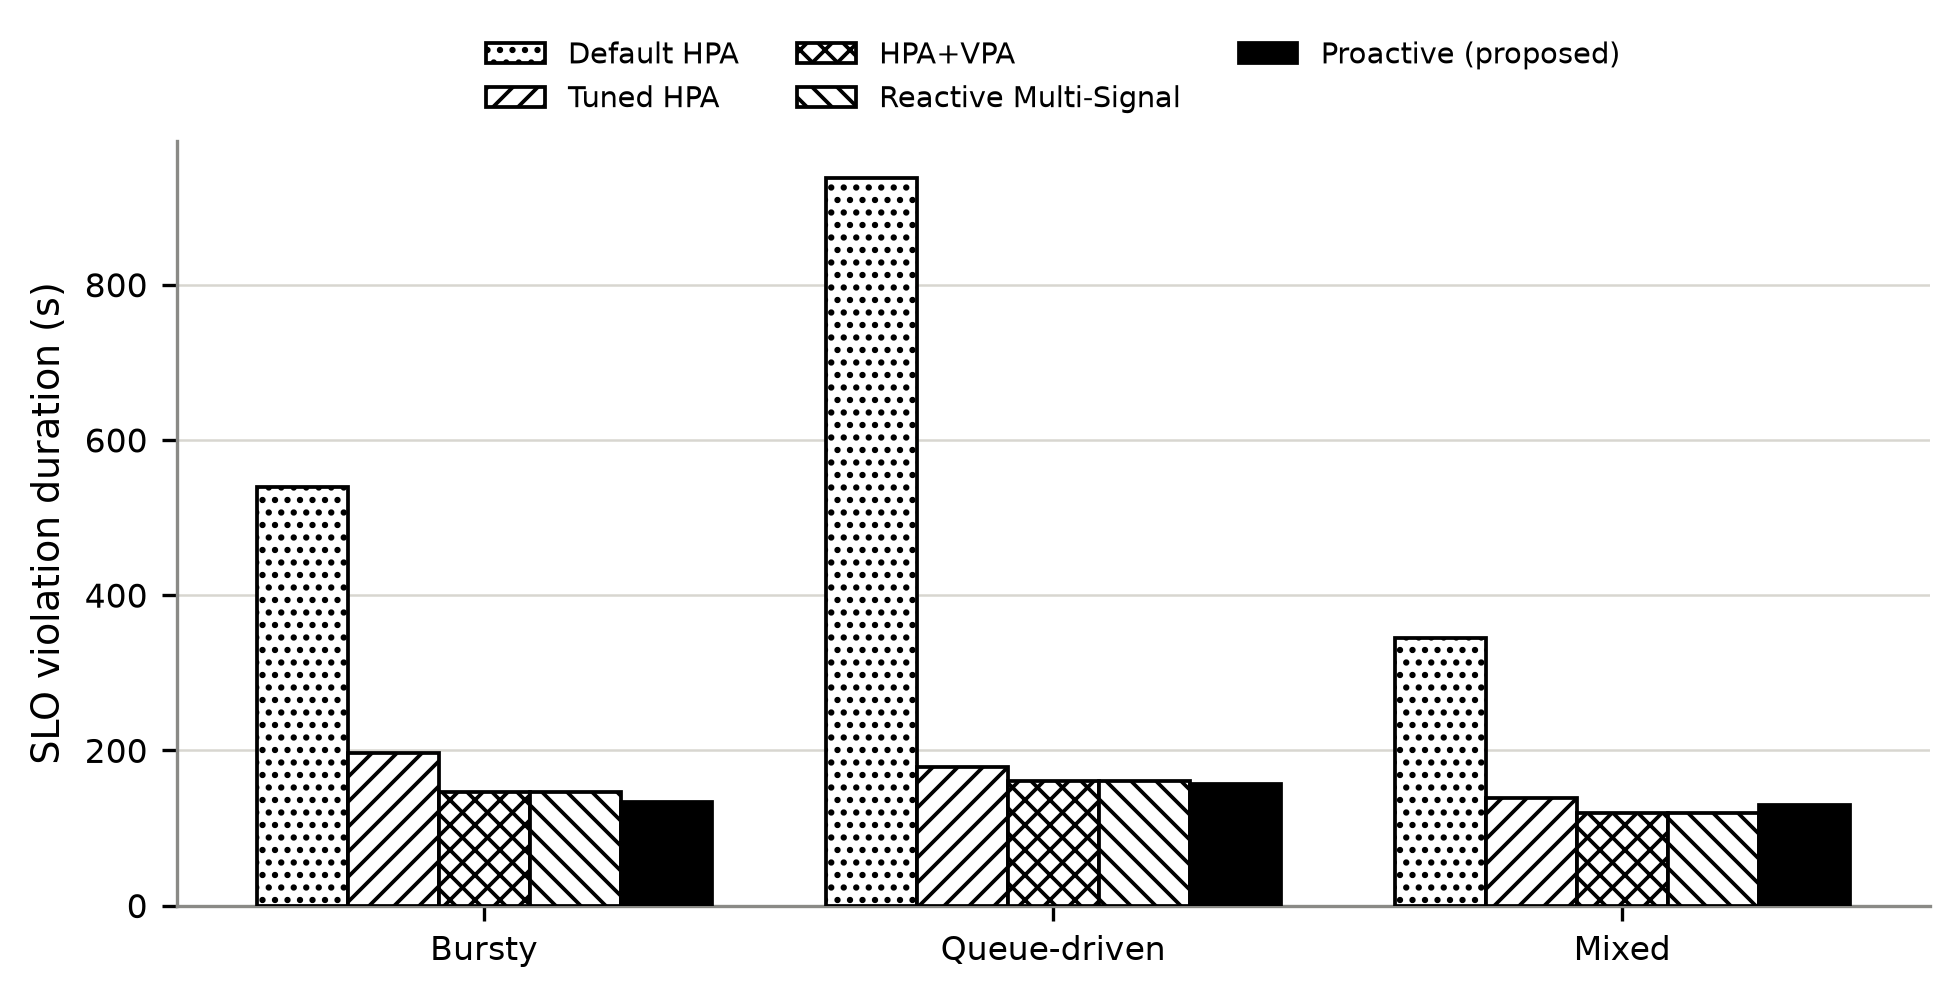
\includegraphics[width=\linewidth]{figures/slo_by_pattern.png}
\caption{SLO violation duration by workload pattern, single seed. HPA+VPA and Reactive Multi-Signal are
numerically \emph{identical} on every pattern (Section~VI-B); the proposed controller is best or
tied-best on bursty/queue-driven and worse on mixed for this seed.}
\label{fig:slo_pattern}
\end{figure}

\subsection{Isolating the Forecasting Contribution}
This is the paper's central comparison. Table~\ref{tab:multiseed} reports mean, standard deviation, and
95\% confidence interval for SLO violation duration across all 24 (pattern, seed) replicates
(Section~V-E), and Figure~\ref{fig:multiseed} visualizes the same data with error bars.

\begin{table}[t]
\centering
\caption{SLO Violation Duration, 24 Replicates (mean $\pm$ std, s)}
\label{tab:multiseed}
\begin{tabular}{lc}
\toprule
Autoscaler & Duration (s) \\
\midrule
Default HPA & $568.6 \pm 225.1$ \\
Tuned HPA & $150.9 \pm 38.6$ \\
HPA+VPA & $125.8 \pm 28.9$ \\
Reactive Multi-Signal & $125.8 \pm 28.9$ \\
\textbf{Proactive (proposed)} & $\mathbf{112.7 \pm 27.5}$ \\
\bottomrule
\end{tabular}
\end{table}

\begin{figure}[t]
\centering
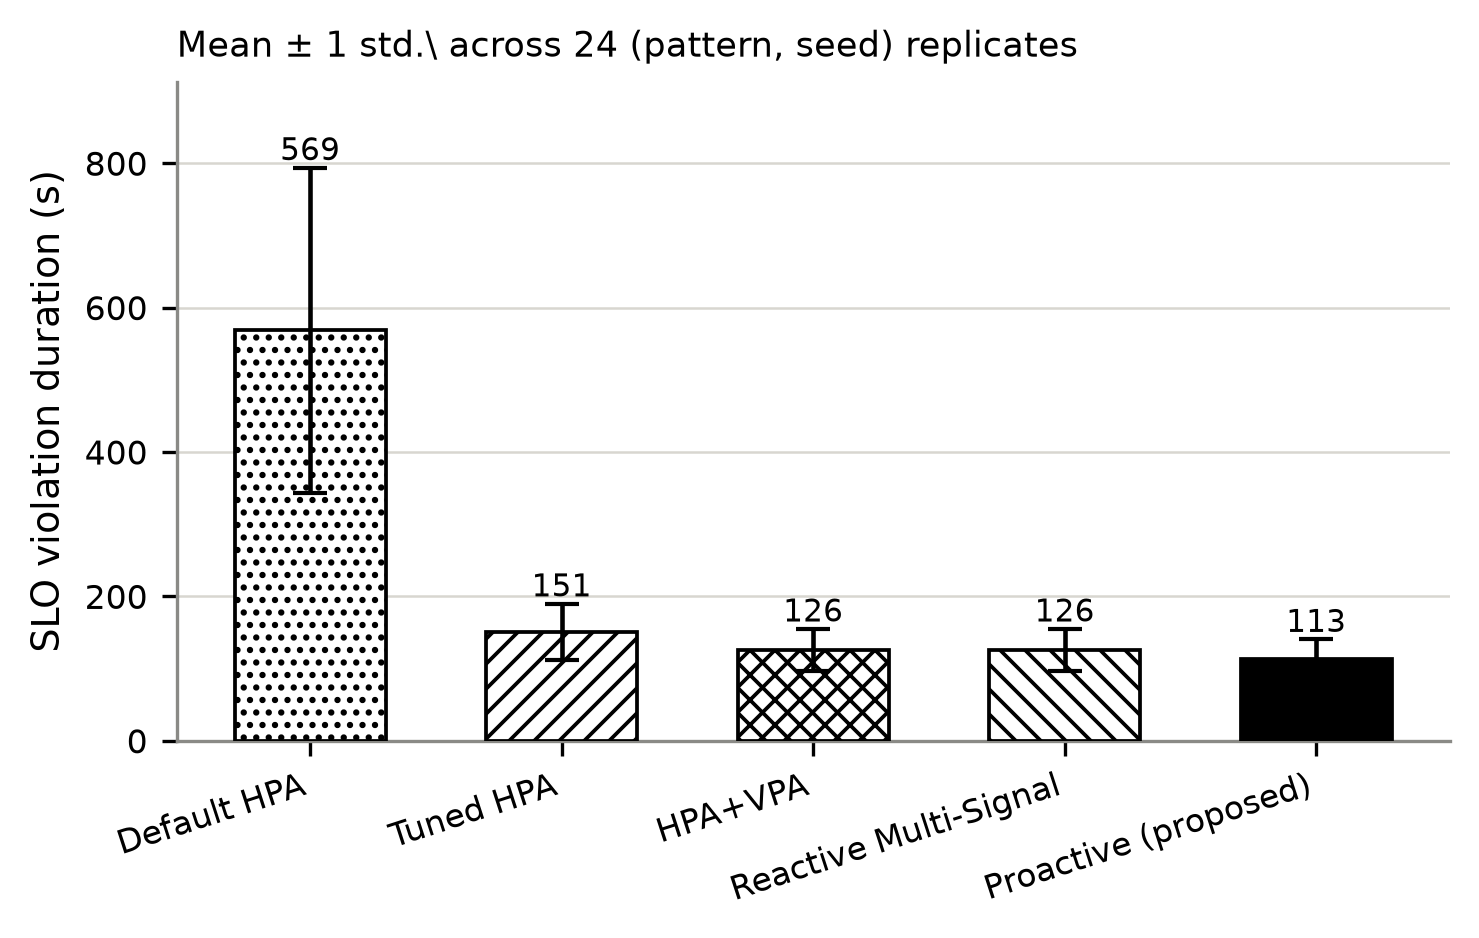
\includegraphics[width=\linewidth]{figures/bar_multiseed_slo.png}
\caption{SLO violation duration, mean $\pm$ 1 std.\ across 24 (pattern, seed) replicates.}
\label{fig:multiseed}
\end{figure}

Two findings follow directly from this table. First, \textbf{HPA+VPA and Reactive Multi-Signal are
numerically identical to three significant figures, on every pattern, at every seed we tested}. Reactive
Multi-Signal has access to two signals HPA+VPA lacks (connection-pool utilization and backlog), yet
never once acts differently. Inspecting the underlying traces explains why: in this simulator, CPU and
p99 latency risk ratios reach values of up to $\approx$1.7$\times$ their thresholds during demand
spikes, while connection-pool utilization's risk ratio rarely exceeds $\approx$1.2$\times$ and RAM's
essentially never crosses 1.0$\times$ -- so the $\max(\cdot)$ risk-fusion rule (Eq.~4) almost always
selects CPU or latency regardless of whether pool/backlog are included. \emph{Widening the signal set
alone, without forecasting, bought nothing in this evaluation.} This is an important negative result:
it directly addresses the possibility that a wider-signal controller's improvement over a
narrower-signal baseline is really just "more signals," since here it demonstrably is not -- the two
controllers with different signal sets but no forecasting are indistinguishable.

Second, the proposed controller's improvement over Reactive Multi-Signal -- the comparison that
isolates forecasting itself, holding the signal set fixed -- is $112.7$ vs.\ $125.8$\,s, a $10.4\%$
reduction, significant under a paired $t$-test ($t=-4.27$, $df=23$, $p=2.9\times10^{-4}$;
Table~\ref{tab:sig}) at statistically indistinguishable infrastructure cost
($5.569$ vs.\ $5.575$ node-hours, $p=0.31$). We report this as the paper's headline forecasting-specific
result rather than the larger-looking 76.9\% figure against Default HPA, which conflates forecasting
with every other design decision (wider signal set, tighter thresholds, different guardrails) relative
to a barely-tuned CPU-only baseline. Critically, as Section~VI-H shows, this significant result holds
only for the \emph{calibrated} damping factor ($\phi=0.97$); at the originally hand-picked value
($\phi=0.85$--$0.9$), the same comparison is not significant ($p=0.12$, and in the wrong direction on
the tuning seeds) -- forecasting's benefit here is real, but it was not free, and it was not present in
this controller's first (uncalibrated) iteration.

\begin{table}[t]
\centering
\caption{Paired Significance Tests, Proposed Controller vs.\ Baseline (24 pairs)}
\label{tab:sig}
\resizebox{\columnwidth}{!}{%
\begin{tabular}{lcc}
\toprule
Comparison & SLO Duration & Node-Hours \\
& (mean diff., $p$) & (mean diff., $p$) \\
\midrule
vs.\ Default HPA & $-455.9$\,s, $p<10^{-4}$ & $+3.34$, $p<10^{-4}$ \\
vs.\ Tuned HPA & $-38.2$\,s, $p<10^{-4}$ & $-0.007$, $p=0.31$ \\
vs.\ HPA+VPA & $-13.1$\,s, $p=2.9\times10^{-4}$ & $-0.007$, $p=0.31$ \\
vs.\ Reactive Multi-Signal & $-13.1$\,s, $p=2.9\times10^{-4}$ & $-0.007$, $p=0.31$ \\
\bottomrule
\end{tabular}%
}
\end{table}

\subsection{Scaling Responsiveness}
Pooled across all 24 replicates, the proposed controller achieves the lowest mean time-to-scale
($21.5$\,s), clearly ahead of Tuned HPA ($28.1$\,s), HPA+VPA and Reactive Multi-Signal (tied at
$30.5$\,s), and Default HPA ($192.3$\,s) -- a larger and more consistent gap than the single-seed
numbers in an earlier iteration of this evaluation suggested, and directly attributable to forecasting:
by the time a reactive controller's trigger threshold is crossed, the calibrated proactive controller
has typically already begun scaling out from its 45-second-ahead forecast. Figure~\ref{fig:timeseries}
visualizes replica trajectories and p99 latency for the bursty workload on the representative seed; the
proposed controller (gold) visibly begins scaling out earlier in the replica-count panel and
correspondingly experiences a shorter latency excursion above the SLO line at each burst.

\begin{figure}[t]
\centering
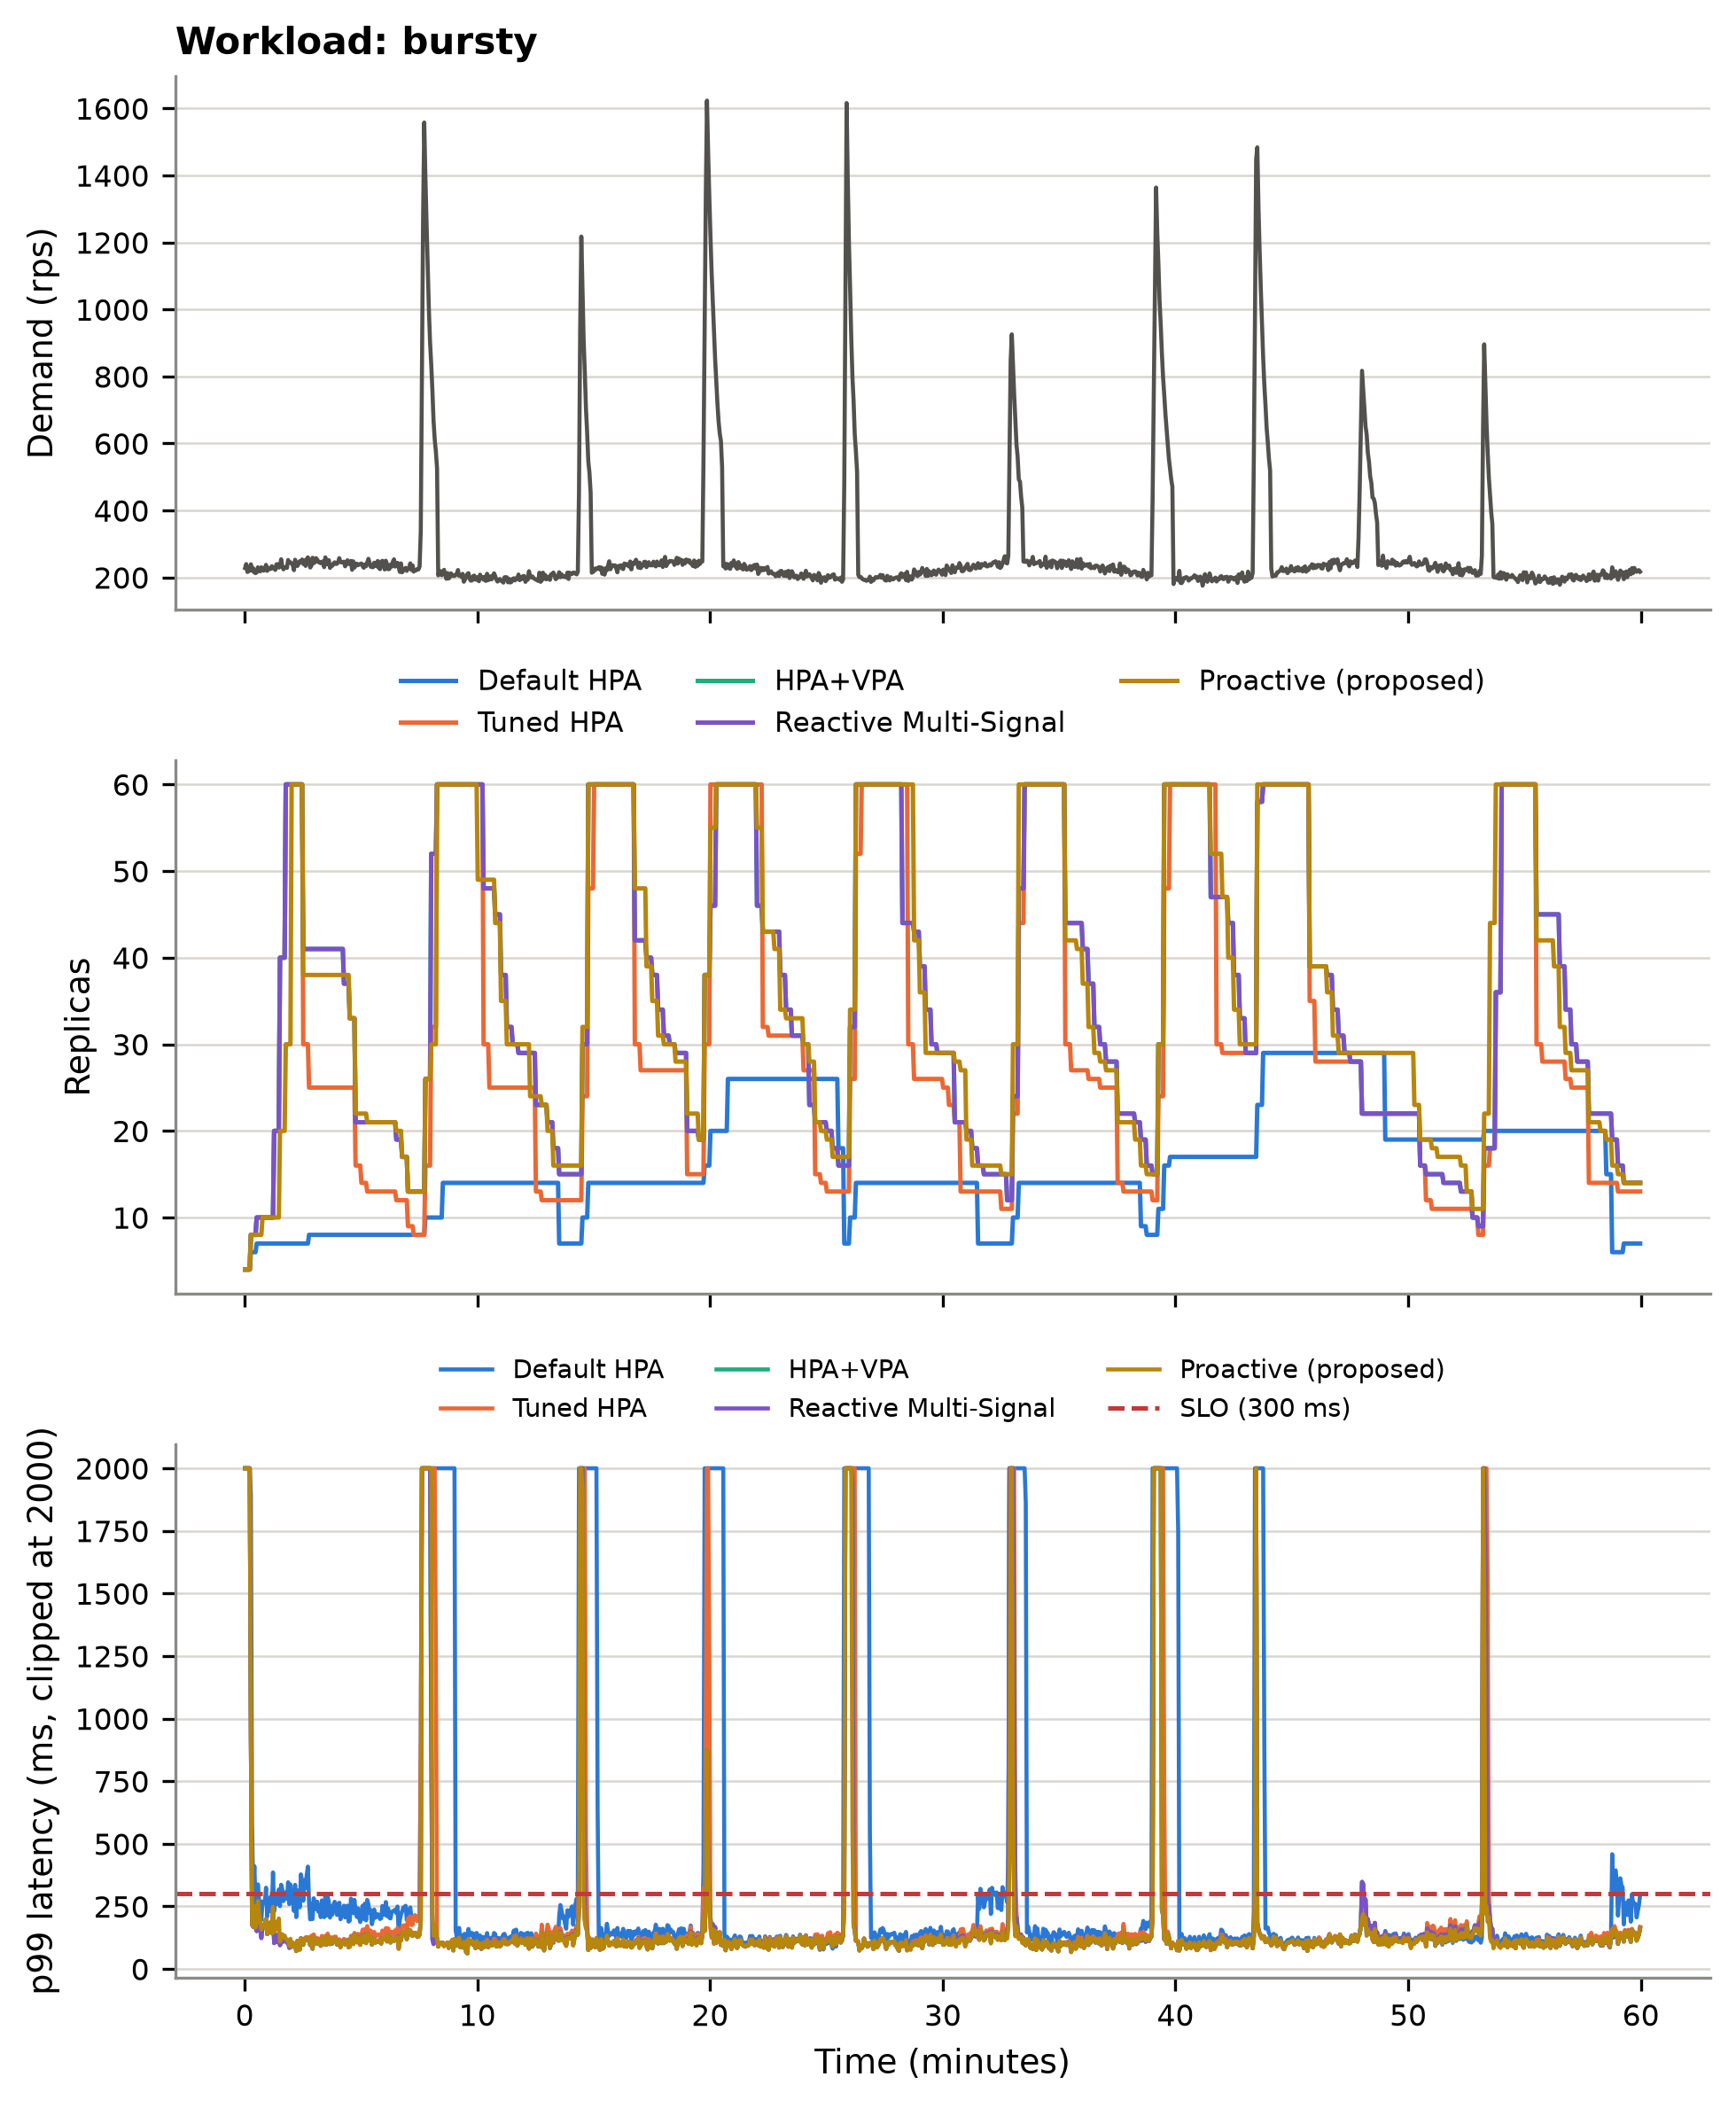
\includegraphics[width=\linewidth]{figures/timeseries_bursty.png}
\caption{Demand, replica count, and p99 latency over a 1-hour bursty-workload run for all five
controllers (single seed). The proposed controller (gold) scales out ahead of each burst and
correspondingly recovers faster below the 300\,ms SLO line (red, dashed). HPA+VPA and Reactive
Multi-Signal (purple) overlap almost exactly.}
\label{fig:timeseries}
\end{figure}

\subsection{Cost Efficiency}
Pooled node-hours (Table~\ref{tab:sig}, right column) show the proposed controller is statistically
indistinguishable in cost from Tuned HPA, HPA+VPA, and Reactive Multi-Signal ($5.569$ vs.\ $5.575$,
$p=0.31$) while delivering significantly better SLO adherence against the latter two -- the improvement
in Section~VI-B is not bought with extra standing capacity. We deliberately do not report cost
reduction relative to Default HPA as a favorable number: Default HPA is cheapest only because it is
severely under-provisioned (Table~\ref{tab:multiseed}), so treating it as a cost baseline would reward
the very under-provisioning the paper argues against.

\subsection{Stability}
Churn counts, pooled across replicates (Figure~\ref{fig:stability}, single-seed version shown), show the
proposed controller is more stable than the reactive HPA+VPA/Reactive Multi-Signal baselines (90.8 vs.\
99.6 churn events/hour) despite reacting to a forecast-based, and therefore individually noisier,
signal set, and only modestly less stable than Tuned HPA (73.2/hour), which reacts to fewer signals and
therefore has fewer opportunities to trigger an action. This suggests the adaptive-blend forecaster's
smoothing remains effective at damping noise-driven thrashing even at the less-damped, calibrated
$\phi=0.97$.

\begin{figure}[t]
\centering
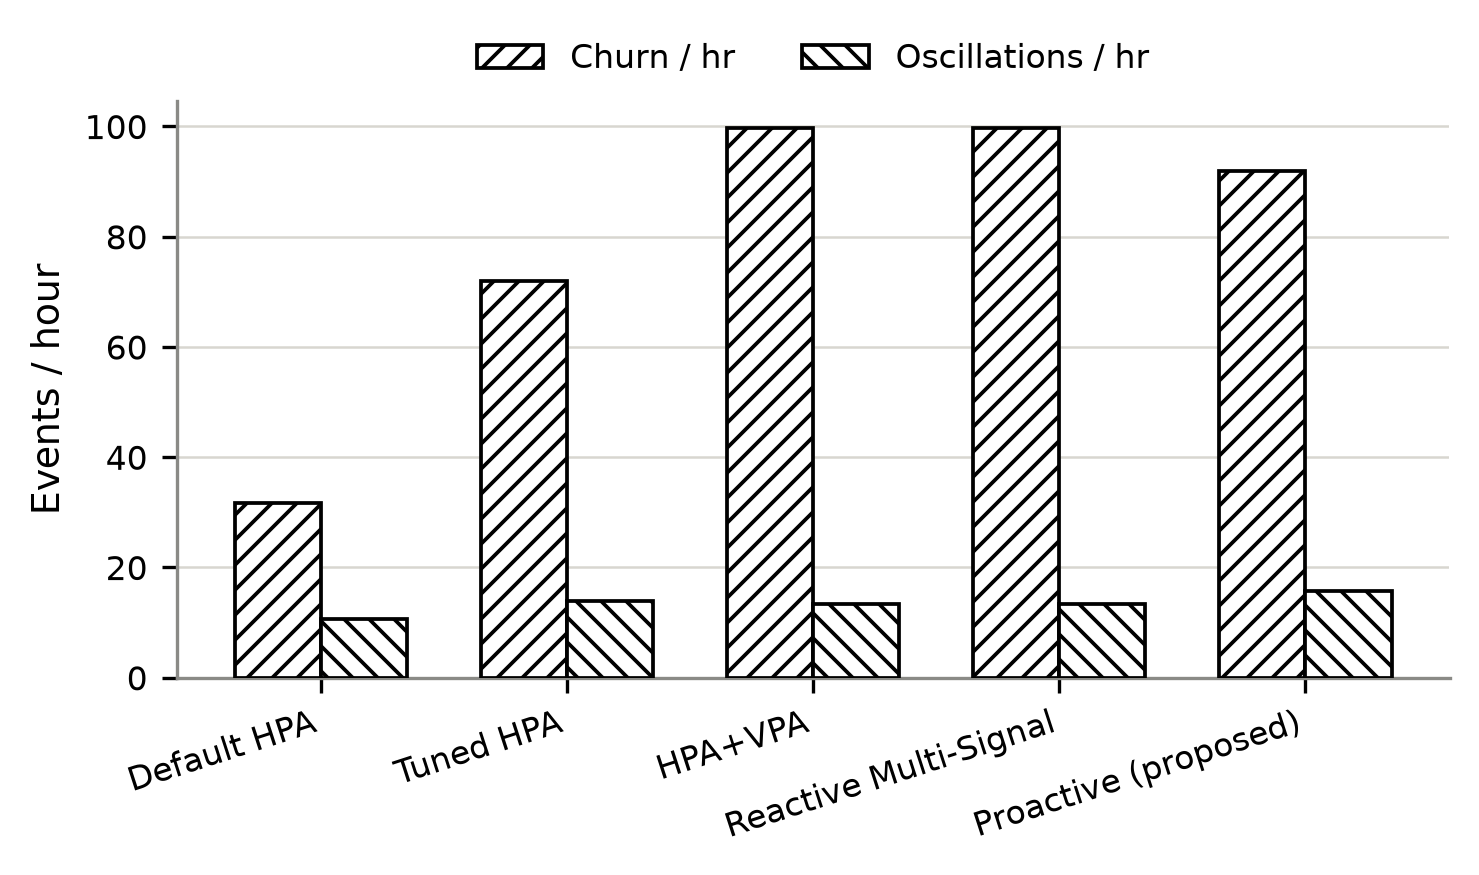
\includegraphics[width=\linewidth]{figures/bar_stability.png}
\caption{Scaling churn and oscillation events per hour, single seed, averaged across workload patterns.}
\label{fig:stability}
\end{figure}

\subsection{Forecast Accuracy}
Figure~\ref{fig:forecast} and Table~\ref{tab:forecast} compare the proposed adaptive Holt/persistence
blend against four classical, training-free baselines: Holt alone, naive persistence, a 20-tick simple
moving average, and a 20-tick linear-drift extrapolator (Section~V-D). Two patterns are visible. First,
\textbf{the adaptive blend improves on Holt alone for three of the four signals} (p99: $82.3\%$ vs.\
$78.5\%$; CPU: $81.6\%$ vs.\ $77.7\%$; connection pool: $88.3\%$ vs.\ $85.7\%$; RAM is roughly flat,
$96.2\%$ vs.\ $96.3\%$, since Holt already wins there and the blend's minimum 5\% weight on persistence
costs it negligibly) -- directly answering the concern that a forecasting layer might barely help at
all for several signals: it still does not \emph{lead} on point-forecast accuracy for p99/CPU/pool, but
it substantially closes the gap to whichever classical method does. Second, and more surprising,
\textbf{naive persistence alone remains the single most accurate point forecaster for the two most
heavy-tailed signals} (p99: $85.9\%$; connection pool: $90.6\%$), ahead of every trend-extrapolating
method including the blend. Linear drift, with no damping at all, is worst on every signal
(RAM $94.5\%$ down to p99 $67.9\%$), confirming that undamped extrapolation is actively harmful here,
not merely unhelpful. RAM is forecast best overall ($96.2\%$, $R^2=0.53$) because its slow,
leaky-integrator dynamics are close to piecewise-linear over the horizon -- the regime trend
extrapolation is designed for.

\begin{table}[t]
\centering
\caption{Forecast Accuracy ($100-\mathrm{SMAPE}/2$, \%), by Signal and Model}
\label{tab:forecast}
\begin{tabular}{lccccc}
\toprule
Signal & Blend & Holt & Persist. & MA(20) & Drift \\
\midrule
p99 latency & 82.3 & 78.5 & \textbf{85.9} & 85.2 & 67.9 \\
CPU & 81.6 & 77.7 & \textbf{83.2} & 81.1 & 70.5 \\
RAM & 96.2 & \textbf{96.3} & 95.5 & 94.8 & 94.5 \\
Conn.\ pool & 88.3 & 85.7 & \textbf{90.6} & 89.8 & 80.0 \\
\bottomrule
\end{tabular}
\end{table}

The natural question this raises -- if persistence is the more accurate point forecaster for p99 and
connection-pool utilization, why forecast them at all? -- is addressed directly in Section~VI-G: point
forecast accuracy (minimizing $|\hat y - y|$) and decision usefulness (correctly anticipating a
threshold crossing early enough to act) are related but not identical objectives, and the two signals
where persistence wins on the former are exactly the two where the windowed classification metrics
below show forecasting still adds detection value the raw accuracy numbers do not reveal.

\begin{figure}[t]
\centering
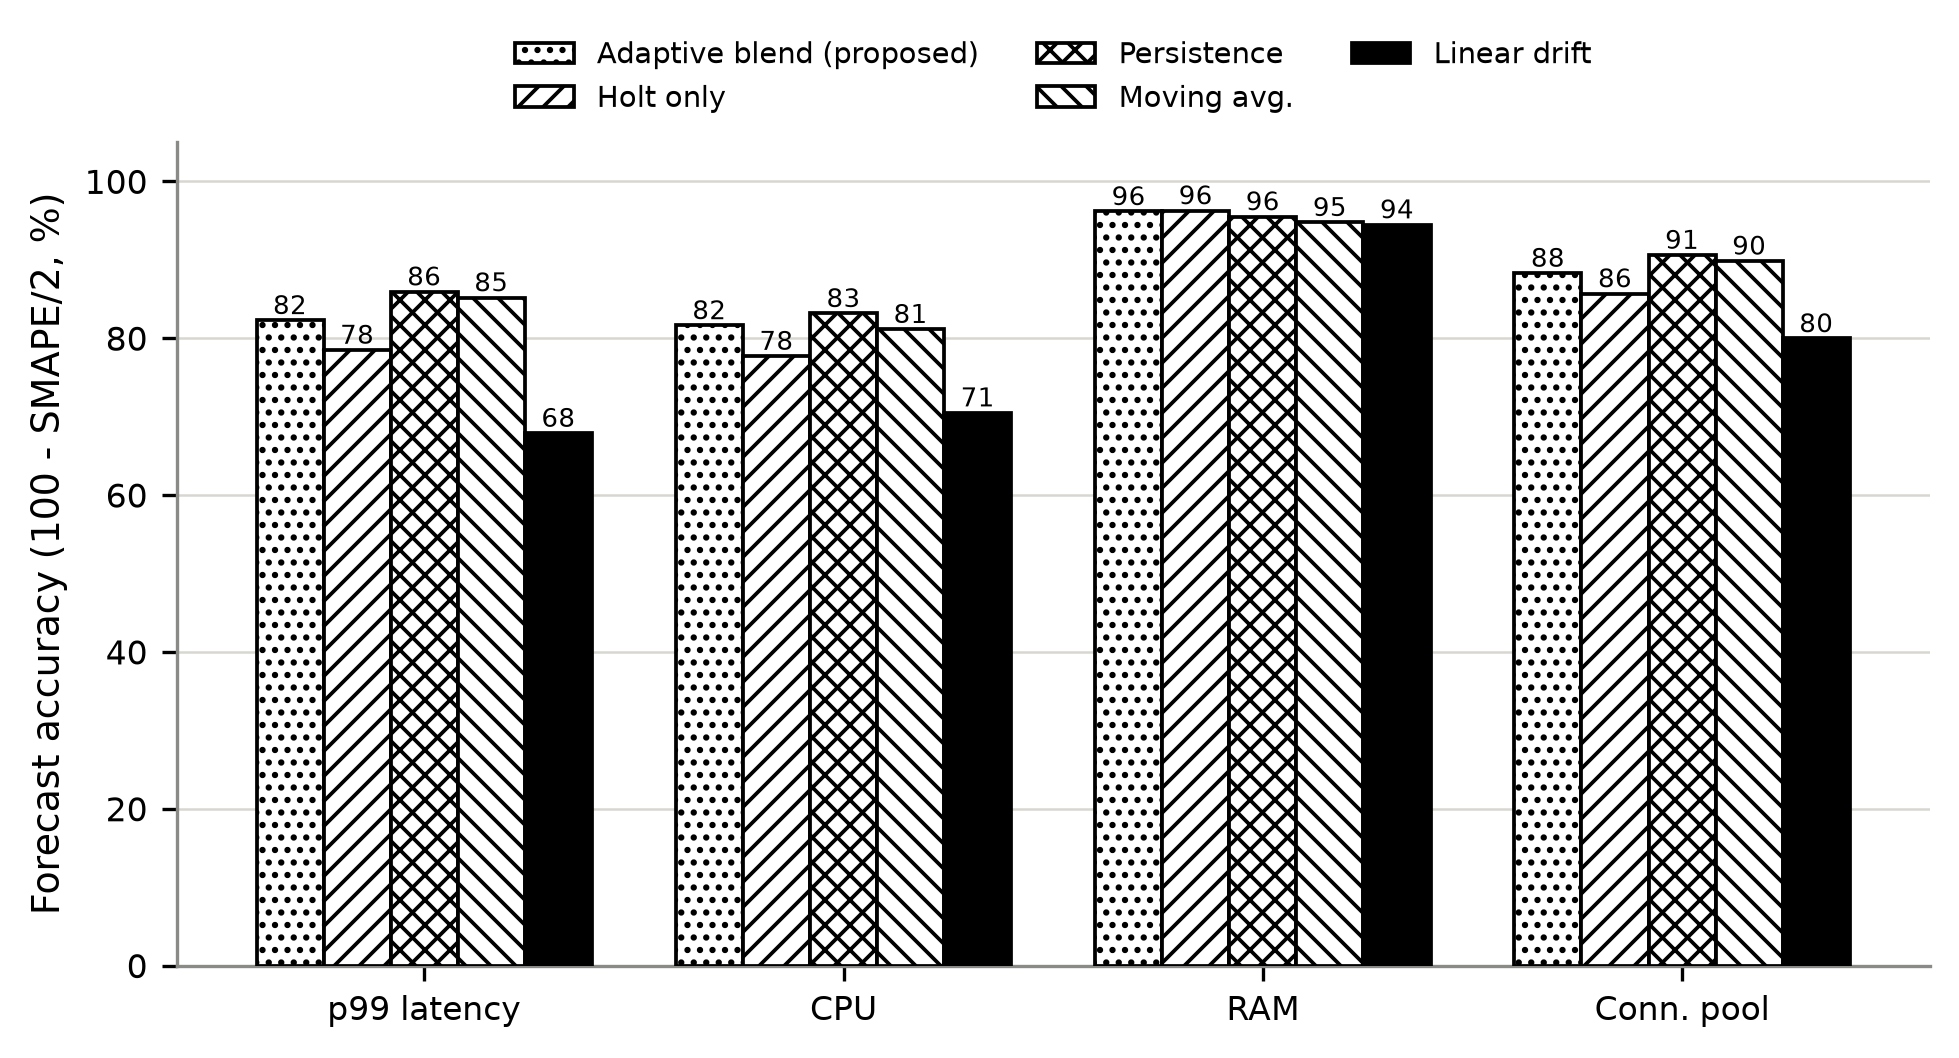
\includegraphics[width=\linewidth]{figures/forecast_accuracy.png}
\caption{Forecast accuracy by signal and model. The adaptive blend (proposed) dominates plain Holt on
three of four signals but still trails persistence on the two heavy-tailed ones (p99, connection pool).}
\label{fig:forecast}
\end{figure}

\subsection{Overload-Prediction Classification}
Table~\ref{tab:class} reports classification quality under the strict, point-in-time definition used by
prior work ("will p99 breach its SLO at exactly $t+h$?"). Both models achieve high raw accuracy
($\approx$93\%), substantially inflated by class imbalance, with weak precision/recall for the positive
(breach) class (F1 $\approx$0.16 for both) -- consistent with the previous section's finding that p99 is
the hardest signal to forecast pointwise at this horizon.

\begin{table}[t]
\centering
\caption{Overload-Prediction Classification, Point-in-Time Definition}
\label{tab:class}
\begin{tabular}{lcccc}
\toprule
Model & Precision & Recall & F1 & Accuracy \\
\midrule
Adaptive blend & 11.9\% & 10.2\% & 16.4\% & 93.8\% \\
Naive persistence & 11.5\% & 10.9\% & 16.7\% & 93.6\% \\
\bottomrule
\end{tabular}
\end{table}

This point-in-time definition, however, is not what a controller deciding whether to act right now
actually needs: it needs to know whether a breach will occur \emph{at any point} before the next
decision opportunity. Table~\ref{tab:class_windowed} reports the same forecasts under that windowed
definition ("will p99 breach at any point in $(t,t+h]$?"). F1 more than doubles for both models (to
0.36 and 0.43 respectively) purely from re-framing the ground truth, with precision reaching 85--94\% --
when either forecaster raises an alarm at the fixed SLO threshold, it is usually right that \emph{some}
breach is coming within the horizon, even though it is frequently imprecise about exactly when.
Sweeping the decision threshold itself (rather than fixing it to the SLO value) and taking the
best-$F_1$ operating point pushes the proposed forecaster to precision $47.9\%$, recall $47.6\%$,
F1 $45.2\%$, with a precision-recall AUC of $0.48$ -- a substantially more favorable and more complete
picture of the forecaster's discriminative power than either fixed-threshold table alone, and the
number we consider most representative of "how good is this forecaster at its actual job."

\begin{table}[t]
\centering
\caption{Overload-Prediction Classification, Windowed Definition}
\label{tab:class_windowed}
\begin{tabular}{lcccc}
\toprule
Model & Precision & Recall & F1 & Accuracy \\
\midrule
Adaptive blend & 84.7\% & 23.3\% & 36.4\% & 89.4\% \\
Naive persistence & 94.2\% & 27.6\% & 42.6\% & 90.5\% \\
\bottomrule
\end{tabular}
\end{table}

\begin{figure}[t]
\centering
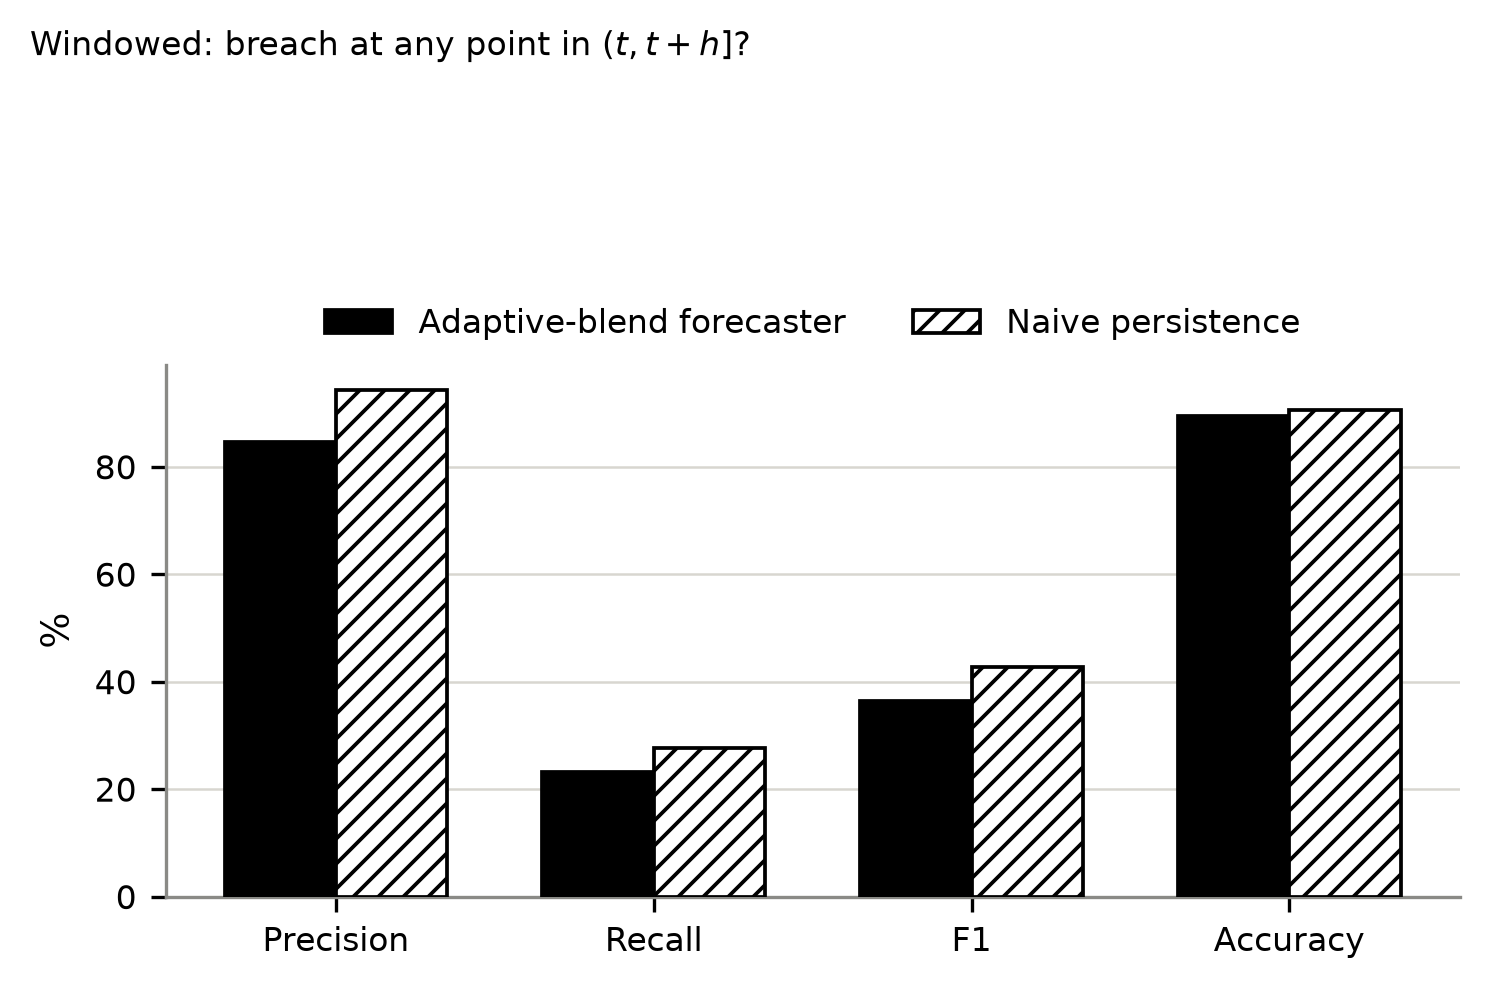
\includegraphics[width=\linewidth]{figures/classification_metrics_windowed.png}
\caption{Windowed overload-classification quality (cf.\ the point-in-time definition,
Table~\ref{tab:class}, under which F1 is $\approx$0.16 for both models). Both forecasters gain
substantially from the windowed re-framing; persistence remains modestly ahead on both definitions,
consistent with the point-forecast-accuracy finding in Section~VI-F.}
\label{fig:class_windowed}
\end{figure}

\subsection{Sensitivity Analysis and Hyperparameter Calibration}
The original iteration of this controller fixed $h=45$\,s and $\phi=0.85$--$0.9$ by hand, matched only
to exceed the simulated node-boot delay, and was not tuned further -- exactly the missing sensitivity
analysis a careful reviewer would ask for. We swept both hyperparameters on the 5-seed \emph{tuning} set
(Section~V-E) and report the paired comparison against Reactive Multi-Signal at every setting.

\textbf{Horizon.} Figure~\ref{fig:sens_horizon} sweeps $h \in \{15,\ldots,120\}$s at the original
$\phi=0.85$. The comparison against Reactive Multi-Signal is never significant across this entire range
($p \in [0.12, 0.20]$), and the point estimate is consistently in the \emph{wrong} direction (proactive
2.3--2.4\,s worse). \textbf{Horizon alone does not rescue the uncalibrated model}: whatever gap exists
between forecasting and not forecasting in this simulator is not explained by having picked the wrong
lead time.

\begin{figure}[t]
\centering
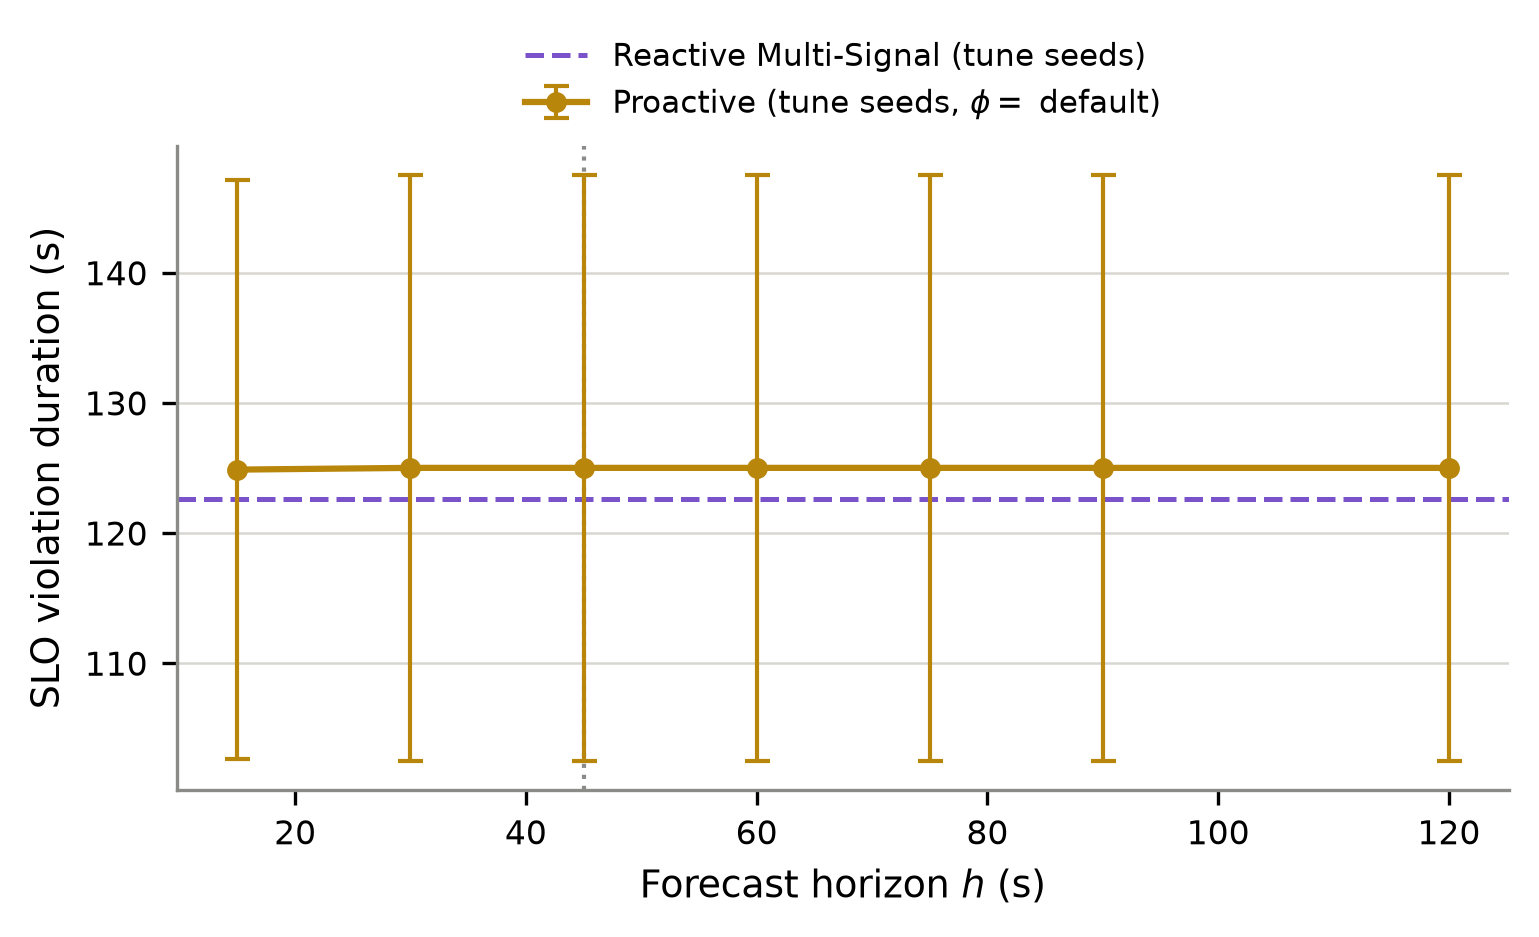
\includegraphics[width=\linewidth]{figures/sensitivity_horizon.png}
\caption{SLO violation duration vs.\ forecast horizon $h$ (tuning seeds, $\phi=0.85$ fixed). Dashed line:
Reactive Multi-Signal baseline. No horizon in this range yields a significant improvement.}
\label{fig:sens_horizon}
\end{figure}

\textbf{Damping factor.} Figure~\ref{fig:sens_phi} sweeps $\phi \in \{0.60,\ldots,0.99\}$ at $h=45$\,s.
Here the picture changes sharply: SLO duration falls monotonically as $\phi \to 1$ (less damping, i.e.\
the trend is allowed to extrapolate further before decaying), from $129.4$\,s at $\phi=0.6$ to
$103.9$\,s at $\phi=0.99$, becoming significantly better than Reactive Multi-Signal from $\phi=0.95$
onward ($p=0.048$) and reaching $p=1\times10^{-4}$ at $\phi=0.99$. We select $\phi=0.97$ rather than the
grid-boundary value $\phi=0.99$: it is unambiguously better than the original $0.85$--$0.9$
($112.5$\,s vs.\ $125.0$\,s, $p=0.010$ against Reactive Multi-Signal) while retaining meaningfully more
damping than the least-damped point tested, reducing the risk of having simply found the edge of a
5-seed grid rather than a genuinely better operating point. Concretely, the damped-trend sum
$\sum_{i=1}^{45}\phi^i$ that bounds how far the trend can extrapolate is $\approx$24 at $\phi=0.97$,
substantially below the undamped limit of 45 that the original design explicitly avoided
(Section~IV-C) and that we did not want to approach even though the grid suggests it would score higher
still on these particular seeds. Notably, node-hours are flat across the entire $\phi$ sweep
($5.56$--$5.59$ throughout), so this is not an accuracy-for-cost trade -- it is a genuine, apparently
non-cost improvement that the original hand-picked value simply left unclaimed.

\begin{figure}[t]
\centering
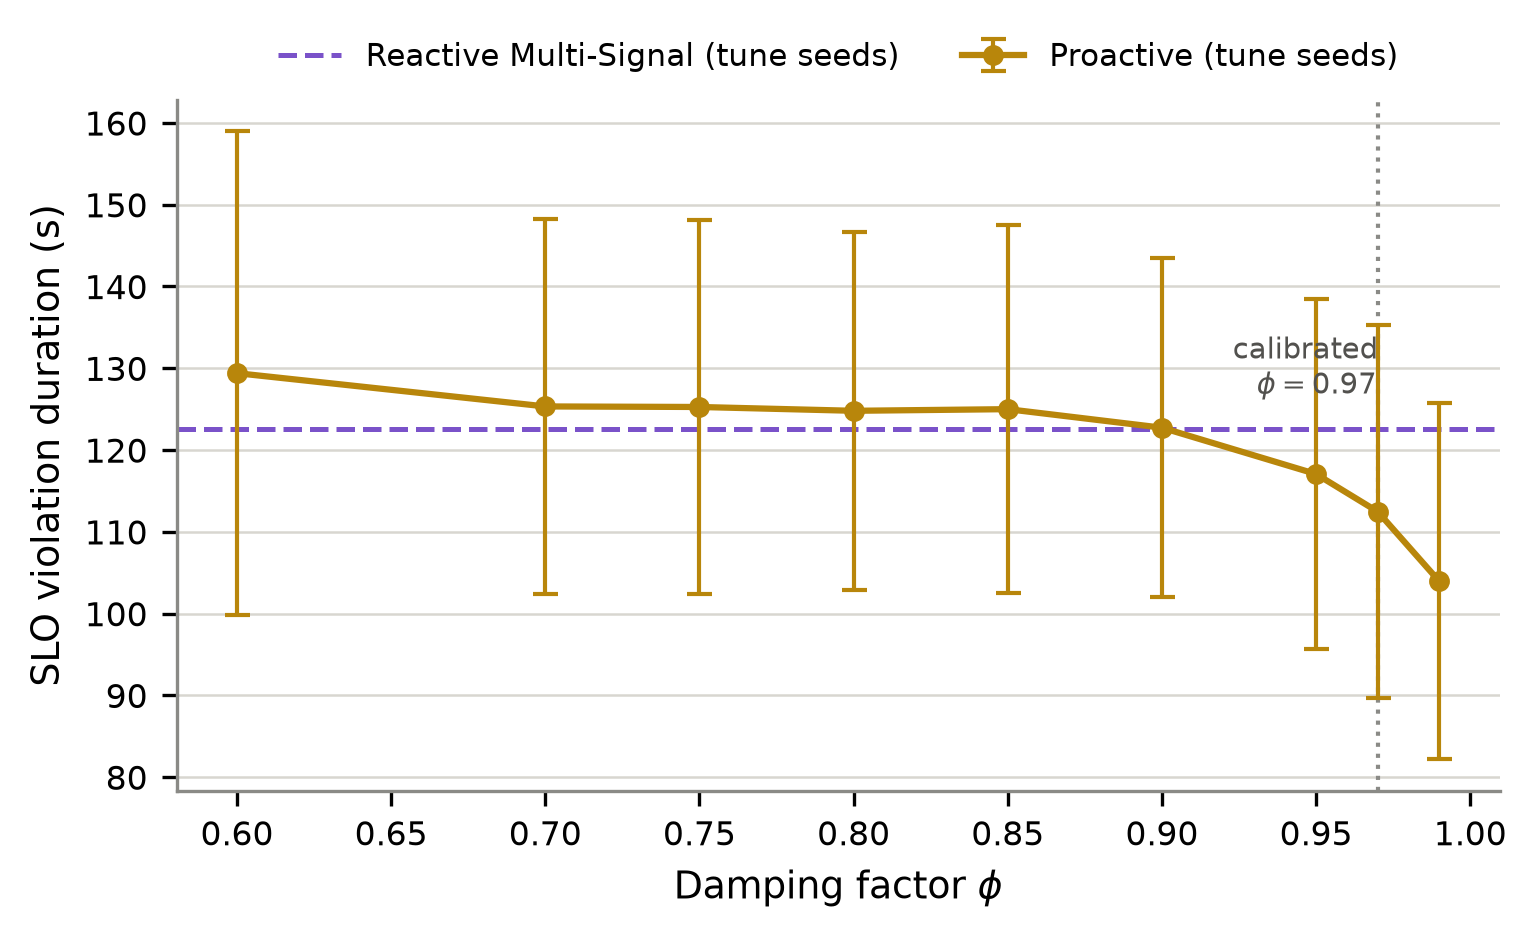
\includegraphics[width=\linewidth]{figures/sensitivity_phi.png}
\caption{SLO violation duration vs.\ damping factor $\phi$ (tuning seeds, $h=45$\,s fixed). Dashed line:
Reactive Multi-Signal baseline. Improvement is monotonic in $\phi$ and becomes significant from
$\phi\approx0.95$; $\phi=0.97$ (dotted) is selected without going to the grid boundary.}
\label{fig:sens_phi}
\end{figure}

\textbf{Held-out validation.} $\phi=0.97$ was selected using only the 5 tuning seeds. Table~\ref{tab:holdout}
re-evaluates it on the 3 disjoint holdout seeds, never used in the sweep above. The calibrated
configuration remains significantly better than both Reactive Multi-Signal ($p=0.014$) and the original,
uncalibrated $\phi$ ($p=0.0022$) on data that played no role in selecting it -- the improvement in
Section~VI-B is not an artifact of hyperparameter overfitting to the seeds used to find it.

\begin{table}[t]
\centering
\caption{Held-Out Validation of $\phi=0.97$ (3 seeds never used for tuning)}
\label{tab:holdout}
\begin{tabular}{lc}
\toprule
Configuration & SLO Duration (mean $\pm$ std, s) \\
\midrule
Reactive Multi-Signal & $131.1 \pm 37.8$ \\
Proactive, original $\phi=0.85$ & $135.2 \pm 39.1$ \\
Proactive, calibrated $\phi=0.97$ & $\mathbf{113.0 \pm 35.6}$ \\
\bottomrule
\end{tabular}
\end{table}

\subsection{Discussion}
Taken together, these results support a narrower and more precisely scoped claim than a blanket
"proactive beats reactive." Three findings drive that scoping. First, widening the signal set alone,
without forecasting, bought nothing in this simulator (Section~VI-B): HPA+VPA and Reactive
Multi-Signal are indistinguishable, because CPU and p99 latency dominate the risk-fusion $\max(\cdot)$
essentially always. Any paper (including an earlier iteration of this one) that credits a wider signal
set for an end-to-end improvement should check this ablation before doing so. Second, forecasting's own
marginal contribution, once isolated this way, is real but was \emph{latent} rather than free: it did
not appear until the damping factor was calibrated by a sensitivity sweep and confirmed on held-out
seeds (Section~VI-H), and it is workload-dependent even after calibration (Figure~\ref{fig:slo_pattern}
still shows the mixed pattern favoring the reactive baselines on the illustrated seed). Third, and most
subtly, forecast point-accuracy and forecast decision-usefulness are not the same thing
(Sections~VI-F--G): persistence remains the more accurate point forecaster for the two most volatile
signals, yet the same forecasts are still useful for the windowed overload-warning task that actually
matters operationally. We view this as a strength of the evaluation methodology rather than a weakness
of the proposed controller: reporting the isolation baseline, the significance tests, the sensitivity
sweep, and the accuracy/classification breakdowns directly, rather than only a single flattering
end-to-end number, is what makes it possible to say precisely which part of the system is responsible
for the observed gains, and how much of the improvement one should expect to survive contact with a
different workload or a different random seed.

\section{Limitations and Future Work}

The most important limitation is unchanged from any simulation-based evaluation and is not resolved by
the statistical rigor added in this revision: the evaluation is conducted entirely within a stylized,
closed-loop simulator rather than on a live Kubernetes cluster (Kind, Minikube, K3s, or a managed
GKE/EKS cluster), and no amount of seeds or significance testing against the simulator's own model
substitutes for that. Multiple seeds show the reported effect is not an artifact of one sampled demand
trace \emph{within this model}; they cannot show the model itself matches a real cluster's latency
distributions, real connection-pool implementations, or real node-provisioning behavior. Reproducing
Section~VI-B's central comparison (Reactive Multi-Signal vs.\ the proposed controller) on a real cluster,
where wall-clock provisioning delay, real interference, and real telemetry noise all differ quantitatively
from this model, is the single most valuable piece of follow-up work and the one we did not do.

Several narrower limitations remain even within the simulator. The forecasting layer's hyperparameters
were calibrated only over forecast horizon and damping factor (Section~VI-H); the Holt smoothing
constants $\alpha,\beta$ were left at their originally hand-picked, per-signal values and were not
included in the sweep, so some further improvement may remain unclaimed there. We evaluated four
classical, training-free forecasting baselines (persistence, moving average, linear drift, Holt) but
deliberately did not implement ARIMA, Prophet, LSTM/GRU, temporal-CNN, or gradient-boosted forecasters:
this was a scope decision consistent with the controller's training-free, $O(1)$-per-tick design goal
(Section~IV-C), not evidence that such models could not do better, and comparing against at least one
trained model on identical traces is a natural extension we leave for future work rather than claim
implicitly by omission. The tune/holdout split (5 vs.\ 3 seeds) is small by machine-learning standards;
it is sufficient to show the calibrated $\phi$ is not pure overfitting to the tuning seeds, but a larger
holdout set would produce a tighter confidence interval on the held-out effect size in
Table~\ref{tab:holdout}. Finally, as Section~VI-A notes, the proposed controller's advantage is not
uniform across workload patterns or individual seeds; combining forecast-driven scaling with a
longer-horizon, backlog-aware adjustment specifically tuned for slowly-building queue-driven surges is a
promising direction, as is extending the multi-signal set to include additional connection-layer
telemetry (e.g., TCP retransmit rate, upstream error rate) as further leading indicators of saturation
-- though Section~VI-B's finding that connection-pool utilization and backlog never actually bind the
existing risk-fusion rule in this simulator suggests any such extension should first check, via the same
Reactive Multi-Signal ablation methodology, whether the new signal changes any decision at all before
crediting it with an improvement.

\section{Conclusion}

This paper set out to answer a single, narrow question: once a multi-signal, SLO-aware autoscaler's
signal set is held fixed, how much does forecasting -- as opposed to simply having more signals -- add?
Answering it required a control condition prior multi-signal autoscaling evaluations do not report
(Reactive Multi-Signal, Section~V-C) and statistical rigor (24 replicated runs, paired significance
tests, and a train/test hyperparameter split) that single-run comparisons cannot provide. The answer we
found is more qualified than a headline "forecasting wins" number would suggest. Widening the signal set
to include RAM and connection-pool utilization, by itself, changed nothing in this simulator: the
reactive baseline with access to those signals is numerically identical to one without them, because
CPU and latency dominate the risk-fusion rule regardless. Forecasting's own marginal contribution is
real -- a statistically significant $10.4\%$ reduction in mean SLO violation duration over the
otherwise-identical reactive baseline ($p<10^{-3}$ pooled, $p=0.014$ on seeds held out from
calibration), at statistically indistinguishable infrastructure cost -- but it was latent rather than
free: it was absent at the forecaster's originally hand-picked damping factor and only emerged after a
sensitivity sweep recalibrated it, a step a hand-tuned forecasting claim can easily skip. We also found
that point-forecast accuracy and decision usefulness diverge for the two most volatile signals (p99
latency, connection-pool utilization), where naive persistence remains the more accurate point
forecaster even though the same forecasts still add detection value once evaluated on the operationally
relevant, windowed overload-classification task rather than a stricter point-in-time one. We believe
this combination -- an isolation baseline, multi-seed statistical testing, out-of-sample hyperparameter
validation, and forecast-accuracy/classification reporting alongside the end-to-end SLO numbers -- is
necessary for a forecasting-based autoscaling claim to be checked and built upon, and we report it in
full precisely so that a reader can disagree with any specific piece of it using the same code and data
we used.

\begin{thebibliography}{00}
\bibitem{ref_base} V. Punniyamoorthy, B. Kumar, S. Saha, L. Butra, M. Palanigounder, A. K. Agarwal,
and K. Kannan, ``An SLO Driven and Cost-Aware Autoscaling Framework for Kubernetes,'' \emph{arXiv
preprint arXiv:2512.23415}, 2025.
\bibitem{ref1} H. Zhou and C. H. Yong, ``Implement HPA for Nginx Service Using Custom Metrics Under
Kubernetes Framework,'' \emph{IEEE Access}, vol. 12, pp. 189722--189734, 2024.
\bibitem{ref3} F. AlQayedi, K. Salah, and M. J. Zemerly, ``Adaptive Cloud Resource Allocation Scheme to
Minimize SLO Response Time Violation,'' in \emph{Proc. IEEE/ACS Int. Conf. Computer Systems and
Applications (AICCSA)}, 2016, pp. 1--5.
\bibitem{ref8} Y. S. D. Reddy, P. S. Reddy, N. Ganesan, and B. Thangaraju, ``Performance Study of
Kubernetes Cluster Deployed on OpenStack, VMs, and Bare Metal,'' in \emph{Proc. IEEE Int. Conf.
Electronics, Computing and Communication Technologies (CONECCT)}, 2022, pp. 1--5.
\bibitem{ref9} S. Roy, R. Dobson, J. Campbell, and S. Kalafatis, ``Efficient Resource Allocation for
Multi-Robot Collaboration via Traffic-Aware Pod Autoscaling,'' in \emph{Proc. 7th Conf. Cloud and
Internet of Things (CIoT)}, 2024, pp. 1--8.
\bibitem{ref11} F. H. L. Buzato and A. Goldman, ``Extending Microservices Performance Optimization
Through Horizontal Pod Autoscaling: A Comprehensive Study,'' in \emph{Proc. IEEE Int. Parallel and
Distributed Processing Symp. Workshops (IPDPSW)}, 2025, pp. 553--562.
\bibitem{ref13} H.-Z. Wu and K.-C. Lai, ``Gradient Descent Based Vertical Auto-Scaling Algorithm for
Microservices,'' in \emph{Proc. 11th Int. Conf. Computing and Artificial Intelligence (ICCAI)}, 2025,
pp. 643--647.
\bibitem{ref14} A. K. Mogal and V. P. Sonaje, ``Predictive Autoscaling for Containerized Applications
Using Machine Learning,'' in \emph{Proc. 1st Int. Conf. Cognitive, Green and Ubiquitous Computing
(IC-CGU)}, 2024, pp. 1--6.
\bibitem{ref15} M. T. Vasumathi, M. Sadasivan, A. V. Asha, V. V. N. P. K. Vema, B. K. Kumar, and
Veeresh, ``AI-Driven Predictive Auto-Scaling for Efficient Microservices Deployment in Cloud Data
Centers Using LSTM and Kubernetes HPA,'' in \emph{Proc. 5th Int. Conf. Expert Clouds and Applications
(ICOECA)}, 2025, pp. 859--864.
\bibitem{ref17} N. Chockalingam, N. Saksena, A. Deshpande, A. Parthasarathy, L. Butra, B. Pothineni,
R. S. Bodala, and A. K. Agarwal, ``Scalable cloud-native architectures for intelligent PMU data
processing,'' \emph{International Journal of Engineering Research \& Technology (IJERT)}, vol. 14,
no. 12, Dec. 2025.
\bibitem{gardner1985} E. S. Gardner Jr. and E. McKenzie, ``Forecasting Trends in Time Series,''
\emph{Management Science}, vol. 31, no. 10, pp. 1237--1246, 1985.
\end{thebibliography}

\end{document}
